\documentclass[12pt]{article}
\usepackage{graphicx}
\usepackage{supertabular}
%\usepackage{subcaption}
\usepackage{subfigure}
\usepackage{multirow}
\usepackage{avant}
%\usepackage[many]{tcolorbox}
\usepackage{varwidth}
\usepackage{color}
\usepackage{tikz}
\usetikzlibrary{backgrounds,arrows,calc,decorations.pathmorphing,backgrounds,positioning,fit,petri}
\topmargin = -15mm
\textheight = 230mm
\textwidth = 155mm
\evensidemargin = 0mm
\oddsidemargin = 0mm
\setcounter{topnumber}{300}
\setcounter{bottomnumber}{300}
\setcounter{totalnumber}{300}
\newcommand{\PISA}{\textsf{PISA} }
\newcommand{\pt}{$p_{T}$ }
\newcommand{\B}{$B$ }
\newcommand{\C}{$C$ }
\newcommand{\bb}{$b\bar{b}$ }
\newcommand{\cc}{$c\bar{c}$ }
\newcommand{\jpsi}{$J/\psi$ }
\newcommand{\pythia}{\texttt{PYTHIA} }
\newcommand{\dcar}{$\rm{DCA}_{R}$ }
\newcommand{\raa}{$R_{AA}$ }
\newcommand{\fvtxz}{$Z_{\rm FVTX}$ }
\newcommand{\bjpsi}{${B} \to J/\psi$ }


\begin{document}

\begin{titlepage}
\begin{center}
 {\LARGE Measurement of the Ratio of B $\to$ \jpsi to \jpsi Production Using Forward Muons From Run 12 proton-proton 510 GeV Collisions} \\
\vspace{15mm}
M.Brooks$^{\mbox{1}}$, J.Huang$^{\mbox{2}}$,X.Jiang$^{\mbox{1}}$,X.Li$^{\mbox{1}}$,S.Lim$^{\mbox{1}}$, M.Liu$^{\mbox{1}}$, M.McCumber$^{\mbox{1}}$, C.da Silva$^{\mbox{1}}$, M.Snowball$^{\mbox{1}}$, H.Van Hecke$^{\mbox{1}}$

\vspace{1cm}

$^{\mbox{1}}$ Los Alamos National Laboratory \\
$^{\mbox{2}}$ Brookhaven National Laboratory  \\
\end{center}

\vspace{2cm}
\date{today}

\vspace{2cm}

%\begin{document}

%\maketitle

%%%%%%%%%%%%%%%%%%%%%%%%%%%%%%%%%%%%%%%%%%%%%%%%%%%%%%%%%%%%

\begin{abstract}

With the addition of the Forward Vertex detector to the PHENIX experiment, it is now possible to precisely measure the vertex position in 
both heavy ion and proton-proton events.  This precision gives the ability to measure the Distance of Closest Approach of all tracks to
the precisely measured vertex, allowing one to discern prompt muons from heavy flavor decays that fly some distance before decaying.
In this paper, Run 12 proton-proton collisions at $\sqrt{s} = $ 510 GeV from the PHENIX experiment will be analyzed using the DCA to 
discriminate between B $\to$ \jpsi and prompt \jpsi's decaying into muons Finally, a ratio of B to \jpsi production by \pt is presented.

\end{abstract}

%%%%%%%%%%%%%%%%%%%%%%%%%%%%%%%%%%%%%%%%%%%%%%%%%%%%%%%%%%%%
\end{titlepage}


\tableofcontents

\newpage

%%%%%%%%%%%%%%%%%%%%%%%%%%%%%%%%%%%%%%%%%%%%%%%%%%%%%%%%%%%%
\section{Introduction}

The B-meson poses a very interesting probe of both QGP and CNM effects in Heavy Ion collisions, however measurements of the B-meson production in pp collisions 
are very necessary for a point of reference to these Heavy Ion measurements. 
Measurement of B-mesons through the \jpsi channel to obtain beauty yields has the advantage that they will show up in the \jpsi mass peak giving a clean selection.
B-mesons have a decay length at rest of 450 $\mu$m that can be used for identification through the Distance of Closest Approach (DCA) in the Forward Vertex Detector (FVTX). 
Between the clean selection of muons coming from the decay of the \jpsi, and the DCA of each muon measured with the FVTX detector, we are able to measure the fraction of 
B-mesons produced with respect to prompt \jpsi's. Using B to \jpsi as a way of establishing the pp measurement reference will allow for future $R_{AA}$ measurements 
of B-mesons as well as provide the opportunity to measure cross sections of B production by leveraging the precision of the FVTX detector.
%The \pt distribution of B-mesons decays through the \jpsi channel in the muon arm acceptance is shown in Figure \ref{fig:Bmeson_jpsi_pt}. 

The Distance of Closest Approach is calculated as the radial displacement in centimeters
of the vector from a track reconstructed in the Forward Vertex Detector (FVTX) from the position of the 
vertex reconstructed using all tracks in the FVTX and VTX.  For muons that are from prompt sources,
such as \jpsi, the calculated DCA distribution will be narrow, with a width representing the resolution of the 
detector.  Muons coming from non-prompt sources, such as B-mesons that fly some distance and then decay,
the DCA will be larger on average than prompt muons, and may be asymmetric about zero.  This difference in
DCA shape provides discrimination power, allowing one to measure the composition of different sources in data,
and is the basis for this analysis.

%\begin{figure}[h]
%\begin{center}
%\includegraphics[width=0.7\linewidth]{Bmeson_jpsi_pt}
%\caption{Transverse momentum distribution of \btojpsi decays at the PHENIX muon arms according to PYTHIA8 simulation.}
%\label{fig:Bmeson_jpsi_pt}
%\end{center}
%\end{figure}


\begin{figure}[h]
\begin{center}
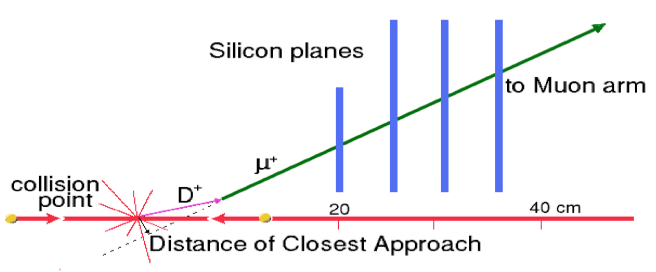
\includegraphics[width=0.7\textwidth,angle=0]{figures/DCA}
\\ \caption{Distance of closest approach.}
\label{fig:DCA}
\end{center}
\end{figure}

\begin{figure}[h]
\begin{center}
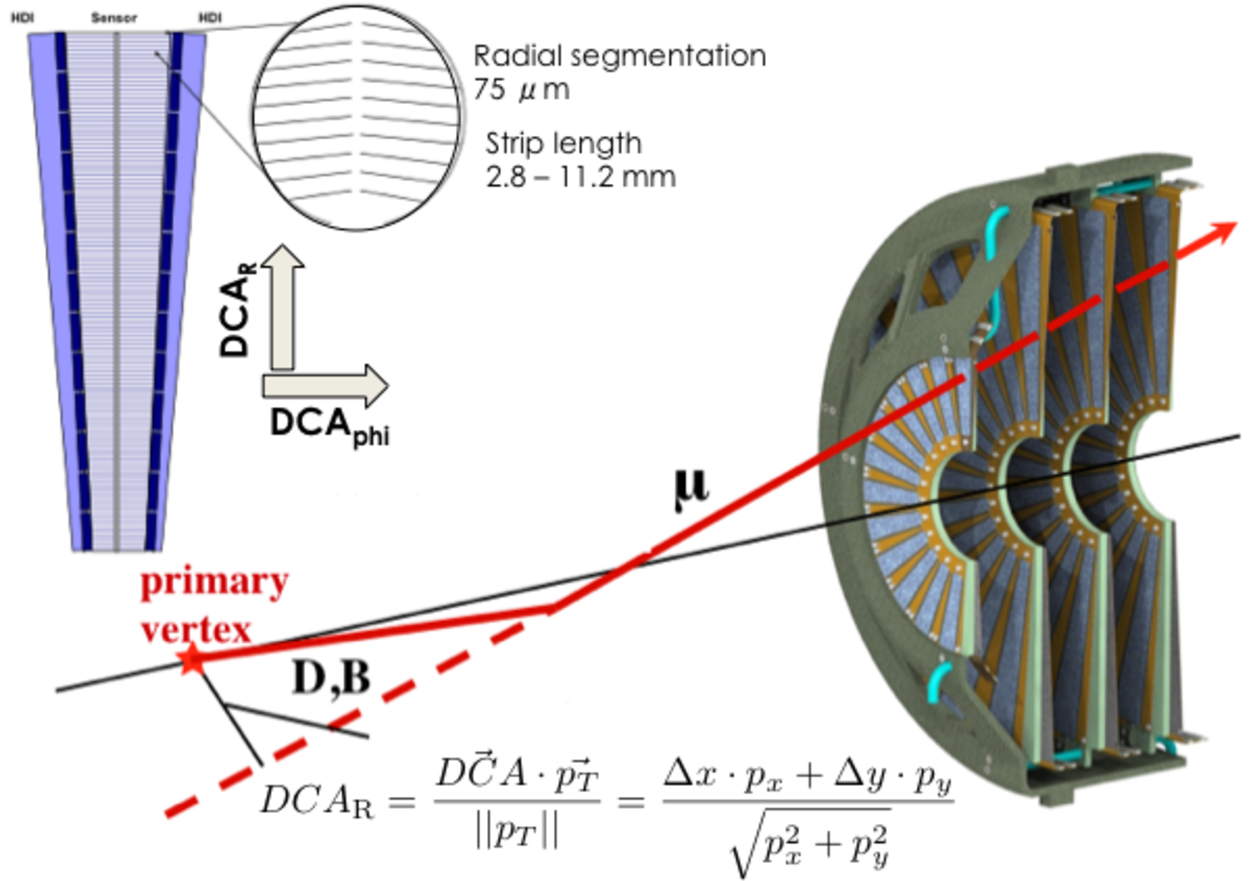
\includegraphics[width=0.7\textwidth,angle=0]{figures/FVTX_DCA_def}
\\ \caption{Distance of closest approach.}
\label{fig:DCA_2}
\end{center}
\end{figure}


The FVTX configuration and how it measures DCA shown in Figures \ref{fig:DCA} and \ref{fig:DCA_2}. The FVTX has a fine radial segmentation of 75 $\mu$m, 
whereas the azimuthal segmentation is determined by the size of the strips, which is between 2.8 and 11.2 mm. Hence, the distance of closest approach needs 
to be projected to the radial direction, or the \pt of the particle. In practice, the resolution of the \pt measurement propagates to the resolution of the \dcar. 
However, it introduces some correlation between \dcar and $DCA_{\rm \phi}$, because the \pt vector is not always perpendicular to the FVTX strips. 

To avoid this additional resolution, a vector from the beam line to the track projection at the first FVTX station of the arm (station 0) is used.
The \dcar analysis of \jpsi dimuon pairs cannot be accomplished purely with the FVTX, because the determination of the \jpsi dimuon crossing requires a 2D vertex detector, that is fine 
resolution in both the radial and azimuthal direction.  The FVTX also does not provide any momentum information.  This information is assigned to the track from the muon tracker, which 
must then be matched to an FVTX track determined to the be the same track. In this analysis we measure the \dcar of select muons in the region of the \jpsi dimuon mass peak. 

This analysis is dedicated to obtaining the fraction of B-meson decays relative to the total \jpsi yield ($f_{\rm B/J/\psi}$) in data obtained during the Run 12 510 GeV proton-proton run.
 As a ratio, the measurement will have minimum systematics impact from the large acceptance and run-by-run trigger fluctuations observed during the 2012 FVTX commissioning run.  
 A cross section for B-meson production is also calculated with both statistical and systematic uncertainties. 


%%%%%%%%%%%%%%%%%%%%%%%%%%%%%%%%%%%%%%%%%%%%%%%%%%%%%%%%%%%%
\section{Datasets and Monte Carlo}
\label{sec:Datasets}

%%%%%%%%%%%%%%%%%%%%%%%%
\subsection{Event Generation}
\label{sec:EventGen}

Pythia 8 has been used to produce all the event level Monte Carlo in this analysis with the CT10 \cite{ref:CT10} parton density function.  
The high luminosity of the Run 12 pp data requires that we simulate multiple vertices in order to capture all effects which may effect
the \dcar.  To simulate this, we must tune the Monte Carlo.  This procedure is described in detail in Sec. \ref{sec:MCTuning}.


\begin{table}[h]
\centering
\caption{Event level Monte Carlo samples}
\begin{tabular}{| l | l | l |}\hline

Type        &    Channel       &    N Events \\ \hline \hline
Signal      &   B $\to$ \jpsi (1 vtx)        &    10M        \\  
Signal      &   B $\to$ \jpsi (2 vtx)        &    4M        \\  
Background   &   \jpsi (1 vtx)       &    10M        \\  
Background   &   \jpsi (2 vtx)       &    4M        \\  \hline

\end{tabular}
\label{tab:EventGen}
\end{table}

%\begin{figure}[h]
%\begin{center}
%\includegraphics[width=0.7\textwidth,angle=0]{figures/}
%\\ \caption{FVTX track multiplicity comparison between Monte Carlo and data.}
%\label{fig:mult_mc_data}
%\end{center}
%\end{figure}

%%%%%%%%%%%%%%%%%%%%%%%%
\subsection{Detector Simulation}
\label{sec:DetSim}
Previous analyses throughout PHENIX have used \PISA which is based on Geant 3 software for simulating particle interactions
with matter in the detector.  While this package is perfectly adequate for most analyses, ones involving extensive hadronic backgrounds
which must be known precisely may suffer from much larger systematics due to the age of the hadron-nucleus interaction software in 
Geant 3.  In order to improve on this, we have implemented PHG3toG4 \cite{ref:PHG3toG4}.  PHG3toG4 is based on the newer C++ based Geant 4 \cite{ref:Geant4}.

Instead of re-writing all of the fortran based geometry code in PISA, we use {\it G4ROOT} \cite{ref:G4ROOT} to export the \PISA geometry to ROOT objects which 
are then read in by PHG3toG4 and translated to Geant 4 geometry with {\it G4ROOT}.  Geant 4 then does all of the particle-material interaction,
and returns the hit results in an identical format to \PISA allowing us to use all of the same DIGI and RECO code downstream. 

PHG3toG4 was validated against both \PISA and Data from Run 12 and 13.  PHG3toG4 hit distributions more closely followed Data than did \PISA's, 
showing that Geant 4 can indeed better simulate particle-material interaction.  The most important difference is Geant 4's ability to better simulate the
showering and scattering of hadrons in thick material such as the absorbers in front of the muon tracking systems.  This effect has historically needed extensive
tuning of the nuclear interaction cross section in \PISA and still resulted in poor agreement with data for hadrons that make it to the third and fourth gap 
in the muon ID system.  Results using this tuning are also susceptible to increasing systematics at high \pt.  Using Geant 4 uses the latest-greatest
nuclear cross sections and propagation code which will reduce these systematics allowing for a more precise measurement.


%%%%%%%%%%%%%%%%%%%%%%%%
\subsection{Run 12 Data and QA Selection}
{\color{red}FIXME}
%%%%%%%%%%%%%%%%%%%%%%%%
\subsubsection{Missing beam center calibration}
In pp runs, beam center position ($x$ and $y$) for each run is used for DCA calculation to get better DCA resolution (Details are shown at~\ref{sec:DCA}).
Among 359 runs of pro. 104 production, 52 runs do not have a beam center position in the database due to bad detector condition of VTX and FVTX.
These 52 runs are rejected to get consistent DCA resolution in the entire data set.

%%%%%%%%%%%%%%%%%%%%%%%%
\subsubsection{MuTr and MuID Performance}

%%%%%%%%%%%%%%%%%%%%%%%%
\subsubsection{FVTX Performance}

%%%%%%%%%%%%%%%%%%%%%%%%
\subsubsection{VTX Performance}


%%%%%%%%%%%%%%%%%%%%%%%%
\subsubsection{FVTX-MuTr Matching}
\label{sec:matching}

A combined FVTX-MuTr track is obtained from production by the module

\begin{verbatim}
offline/packages/fvtxoo/modules/mMutKalFitWithSiliReal.
\end{verbatim}

The combined fit and its $\chi^2$ is calculated by refitting all hits from MuTr and FVTX and the FVTX-MuTr track combination with the smallest $\chi^2$ is chosen. Whereas the calculation 
procedure is the best possible using all hit information; event mixed matches and multiple matches per MuTr track are not implemented. These features become fundamental for analyses in 
environments with large occupancy as explained later in Section \ref{sec:mismatch}. An after burner module is implemented at

\begin{verbatim}
offline/AnalysisTrain/picoDST_object/mFvtxMuTrAssociation
\end{verbatim}

\noindent using the MWG and FVTX tracklet information available from production to calculate multiple same and mixed event FVTX-MuTr matches. 
The association procedure in this module is the following:

\begin{enumerate}
	\item MuTr track parameters are used as input to a GEANT-based track projector
	\item MuTr track is projected atthe Z positions:
	\begin{itemize}	
		\item $|z_0|$=40 cm at the FVTX station 4
		\item $|z_1|$=189.1 cm at MuTr station 1
		\item $|z_2|$=70 cm at the midle of the absorber
	\end{itemize}
	\item FVTX track parameters are used as input for the same track propagator and projected at the same Z positions
	\item radial and azimuthal residuals, momentum vectors and corresponding uncertainties are calculated at each matching plane
	\item the $\chi^2$ of the matching is calculated from the sigmalized residuals
\end{enumerate}

\begin{eqnarray}
\label{eq:match_chi2}
	\textrm {match } \chi^2 = \sum_{zi} && \left(\frac{r_{FVTX}(zi)-r_{MuTr}(zi)}{\sigma R_{fvtx-Mutr}(zi)}\right)^2\\\nonumber
	&+& \left(\frac{phi_{FVTX}(zi)-phi_{MuTr}(zi)}{\sigma\phi_{fvtx-Mutr}(zi)}\right)^2\\\nonumber
	&+& \left(\frac{pr_{FVTX}(zi)-pr_{MuTr}(zi)}{\sigma pR_{fvtx-Mutr}(zi)}\right)^2\\\nonumber
	&+& \left(\frac{p\phi_{FVTX}(zi)-p\phi_{MuTr}(zi)}{\sigma p\phi_{fvtx-Mutr}(zi)}\right)^2
\end{eqnarray}

The matching criteria also includes the track $\chi^2$ of the MuTr and FVTX:

\begin{equation}
\textrm{chi2\_fvtxmutr} = \frac{1}{\rm NDF} \left[ \textrm{match } \chi^2 + \textrm{MuTr track } \chi^2 + \textrm{FVTX track } \chi^2 \right].
\end{equation}

The matching has 2 spacial plus 2 momenta coordinates for each one of the three matching planes. Each FVTX and SVX hit has two coordinates in the fit. The Kalman filter 
fitting uses 5 parameters. Therefore, the number of degrees of freedom is

\begin{eqnarray}
	NDF &=& NDF_{\rm match} + NDF_{\rm MuTr} + NDF_{\rm FVTX}\\\nonumber
	NDF_{\rm match} &=& 12\\\nonumber
	NDF_{\rm MuTr} &=& nhits_{\rm MuTr} - 5\\\nonumber
	NDF_{\rm FVTX} &=& 2*(nhits_{\rm FVTX} + nhits_{\rm SVX}) -5.
\end{eqnarray}

The standard deviations $\sigma R$, $\sigma \phi$, $\sigma pR$ and $\sigma_{p\phi}$ in Eq. \ref{eq:match_chi2} are calculated from the MuTr and FVTX projection covariant matrices. The 
correctness of this calculation was studied using mismatch subtracted residual distributions (see Section \ref{sec:mismatch}) in real data and pure simulated samples. The studies showed that 
the calculation is not always correct, giving uncertainties which variate up to 50\% from the observed matching plane residuals. The problem seems to come from the calculation of the original 
track covariant matrices but no further investigation was developed to track down the source of the incorrectness. 

The $\sigma$ parameters were then obtained by fitting the momentum dependence of the residuals in each matching plane using simulated data. The general fitting function describing the 
one standard deviation of the residuals is a polynomial 

\begin{equation}
	\sigma_{r,\phi,pr,p\phi}(zi) = a + b/{\rm mom} + c/{\rm mom}^2.
\end{equation}

All FVTX-MuTr matches with chi2\_fvtxmutr $<$3 are accepted for the \dcar analysis. A single MuTr track can match more than one FVTX track. Section \ref{sec:matching} describes how to 
statistically remove the mismatch contribution of the \dcar distributions. The result of the re-association procedure is compared to the the association obtained during production, which uses 
all hits information, is shown in Figure \ref{fig:reassociation_comparison}. The matched $\chi^2$ provided by the re-association module is slightly smaller than the one from production. 

%\begin{figure}[h]
%\begin{center}
%\subfigure[]{\resizebox{7cm}{!}{ 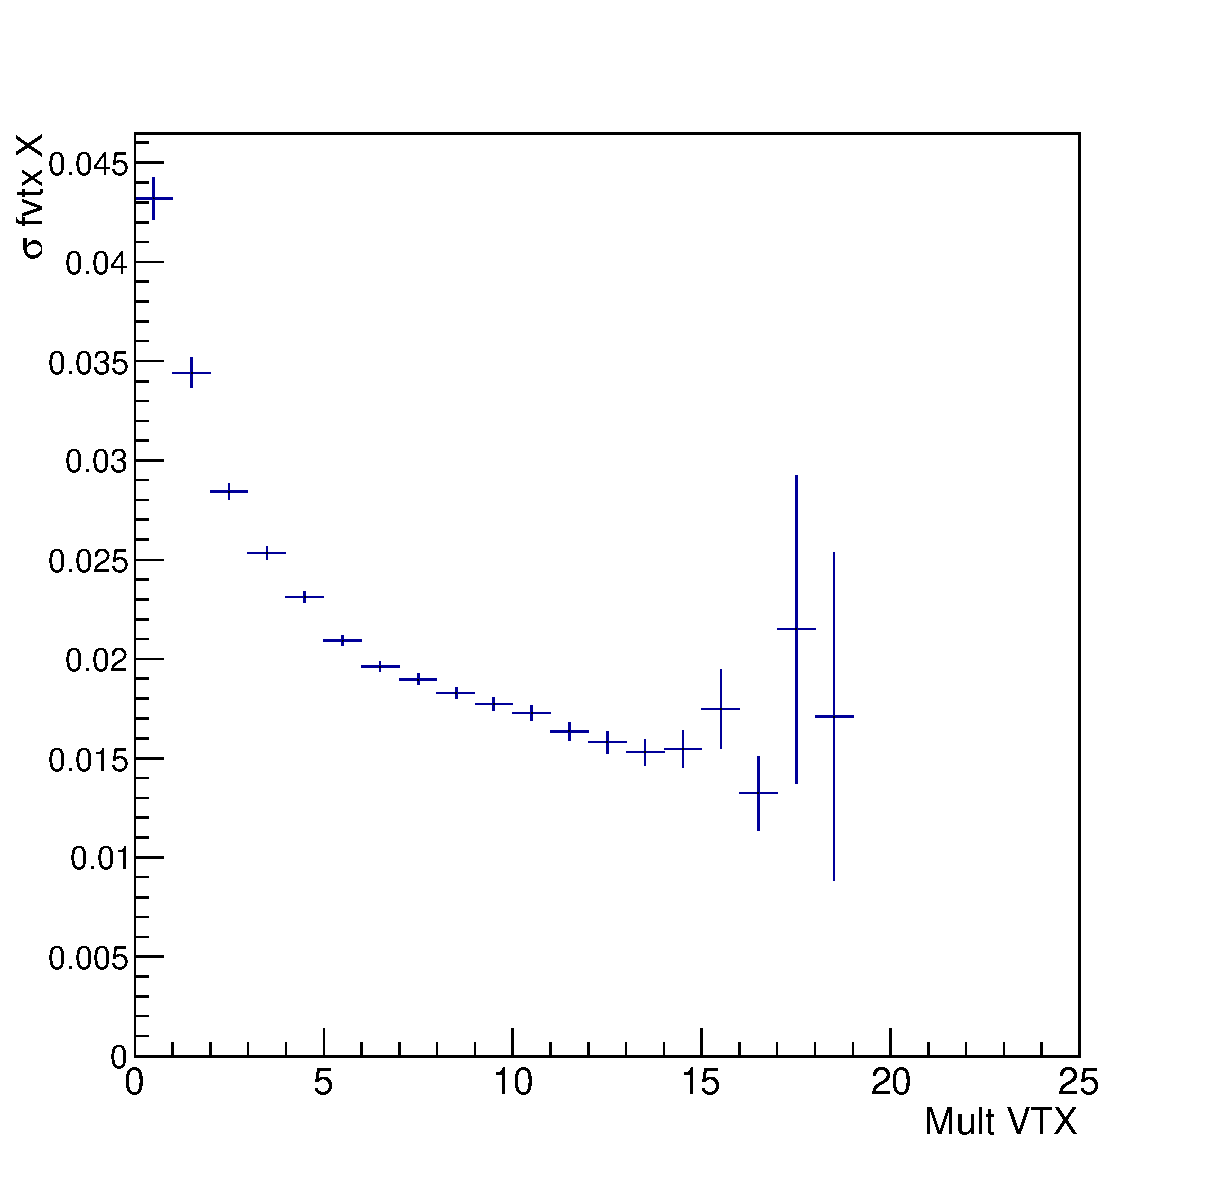
\includegraphics{Figures/fvtxX_v_MultSVX_fit}}} 
%\subfigure[]{\resizebox{7cm}{!}{ 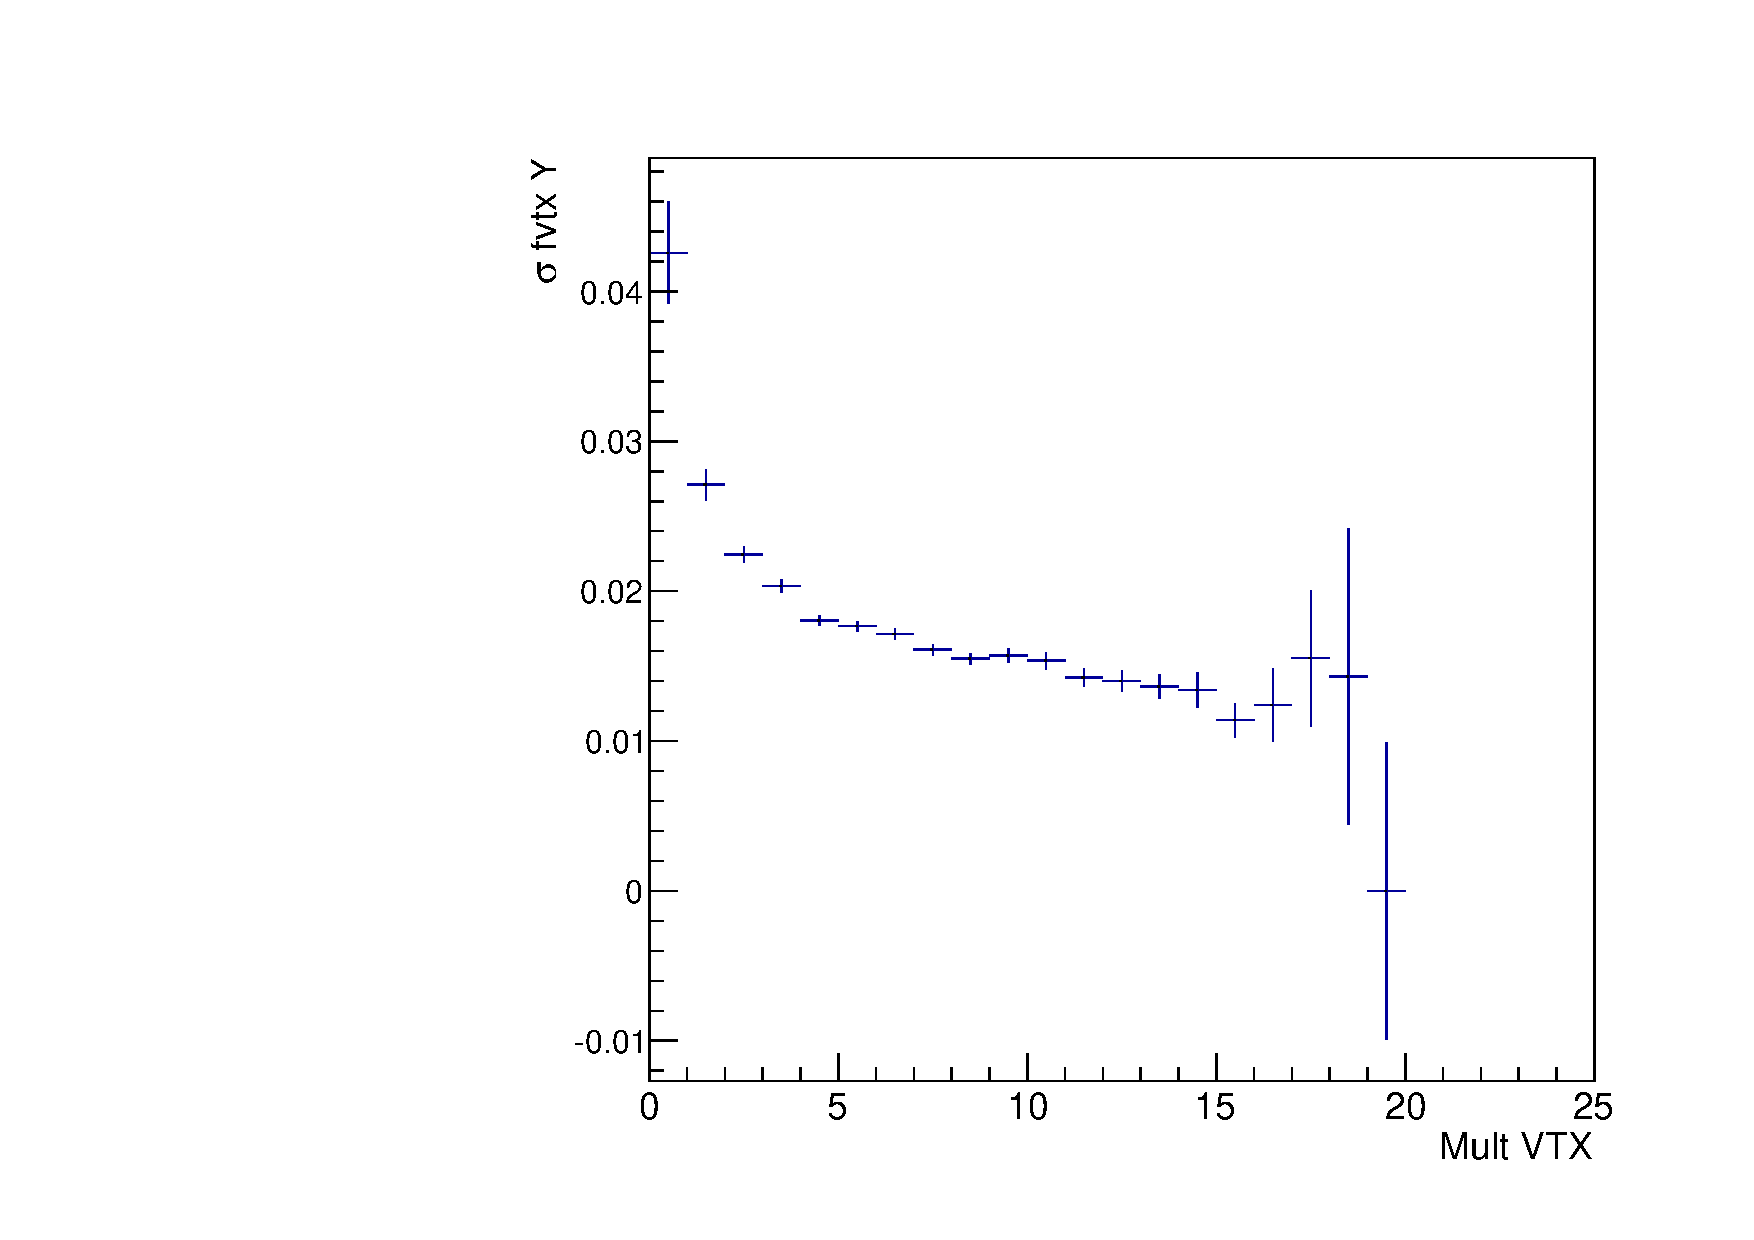
\includegraphics{Figures/fvtxY_v_MultSVX_fit}}} \\
%\\ \caption{Comparison of \dcar with and without re-association (left) and $\chi^{2}$ with and without re-association (right) in MC.}
%\label{fig:reassociation_comparison}
%\end{center}
%\end{figure}


The chi2\_fvtxmutr cut comprises all matching cuts such as \verb|dr_fvtx| and \verb|dphi_fvtx|. However, biases in \dcar at the edges of the FVTX acceptance can happen as discussed in 
Section \ref{sec:fiducial cuts}. In order to minimize these effects the difference between the FVTX and MuTr $\phi$ angle projection at FVTX station 4 needs to be smaller than 100 mrad 
(\verb|abs(dphi_fvtx)<0.1|)


%%%%%%%%%%%%%%%%%%%%%%%%
\subsubsection{Fiducial Cuts}
\label{sec:fiducial cuts}



%%%%%%%%%%%%%%%%%%%%%%%%%%%%%%%%%%%%%%%%%%%%%%%%%%%%%%%%%%%%
\section{DCA Resolution}
\label{sec:DCA}

The resolution of the \dcar of a muon to the primary vertex is governed by the convolution of two main pieces: track resolution and vertex resolution.
The track resolution depends on momentum of the particle through the FVTX and muon tracking system.  The particle must have enough momentum to pass through 
the FVTX, the ~80 cm of steel absorber behind the FVTX, the muon cathode strip chambers and resistive plate chambers, as well as the alternating absorber and muon ID
spectrometers.  Low momentum tracks will suffer from greater losses in the absorber layers as well as more deviation from multiple scattering, lowering the quality of the track
measurement.  At the same time, these low momentum particle have a larger sagita, bending further in the magnetic field of the muon tracking system.  Figure \ref{fig:MuonTrackDCA}
shows the \dcar resolution of these tracks versus muon total momentum. This figure shows purely the tracking resolution component of the total \dcar resolution.

\begin{figure}[h]
\begin{center}
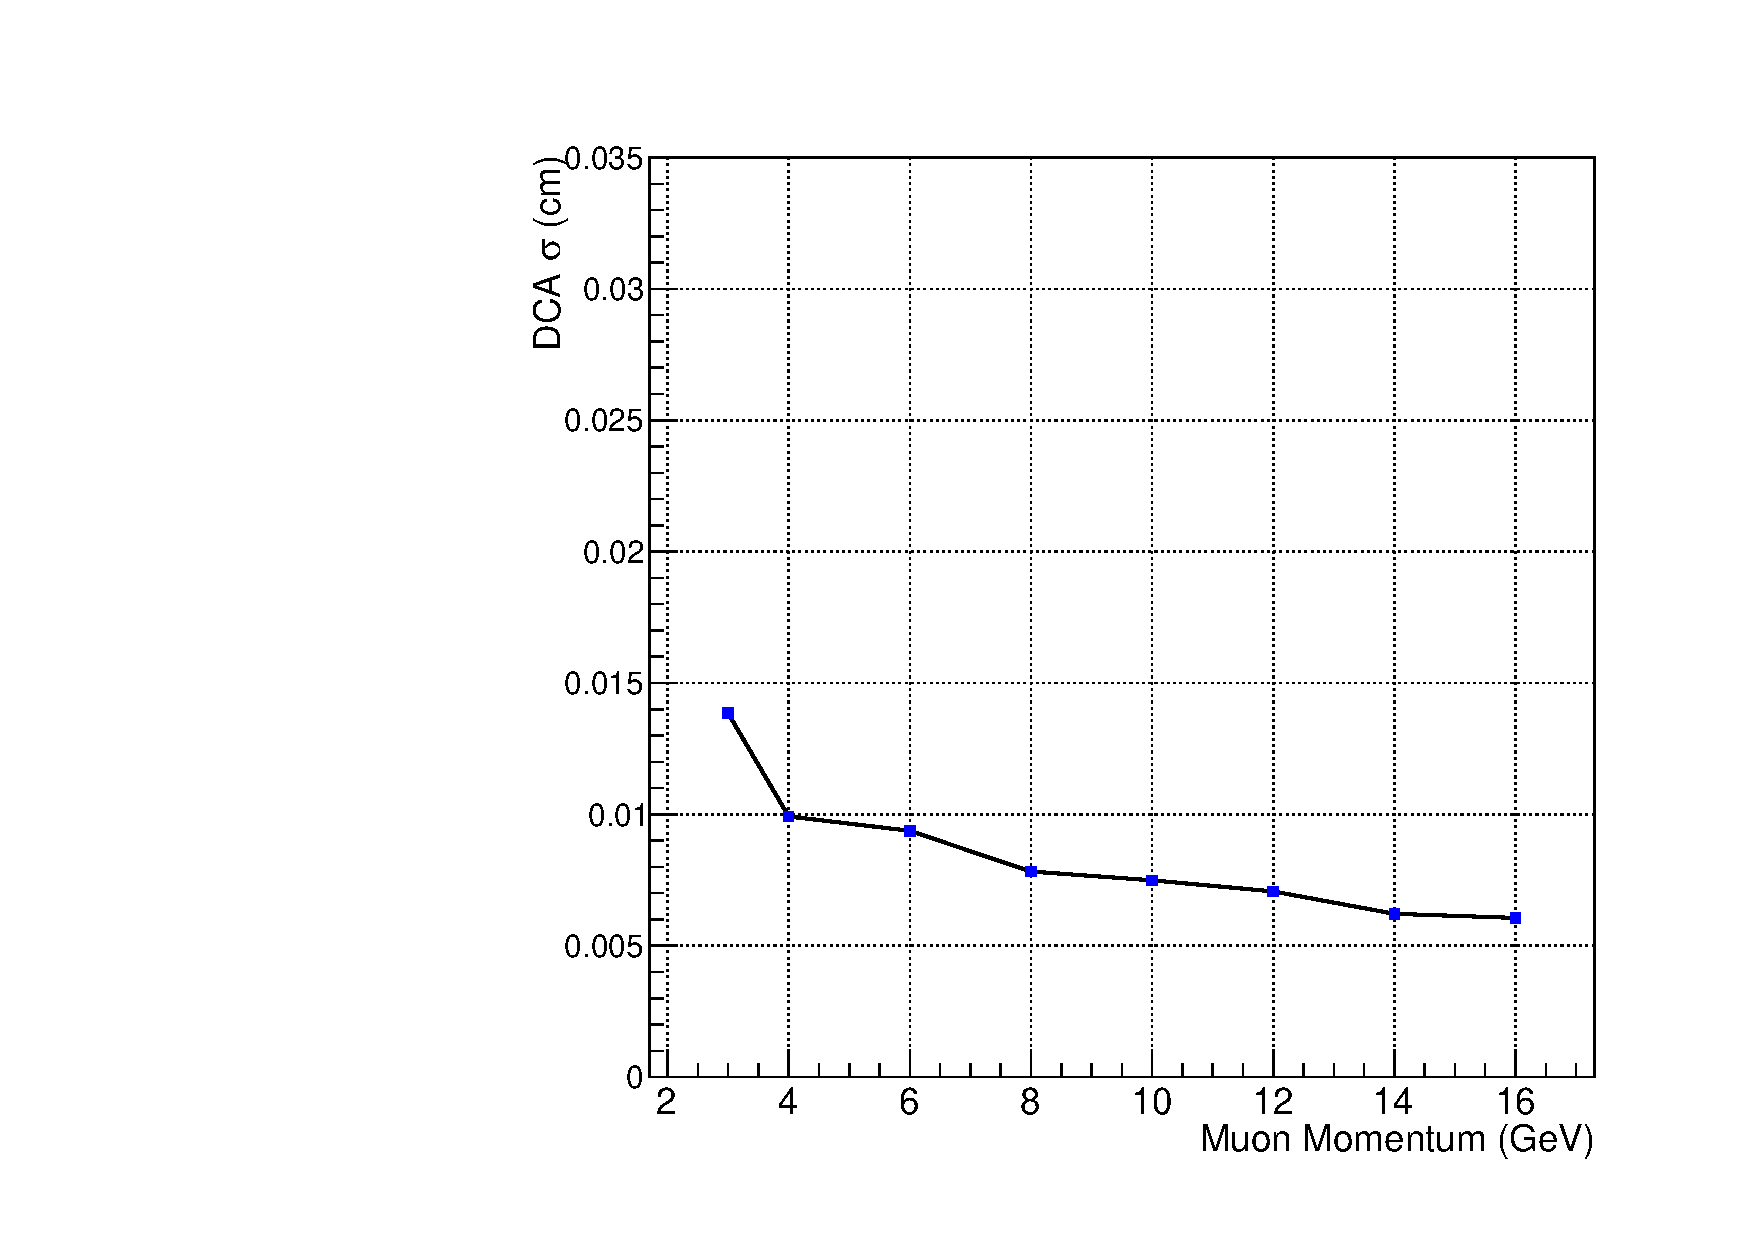
\includegraphics[width=0.6\textwidth,angle=0]{figures/SingleMuon_SigmaVMomentum}
\\ \caption{Distance of closest approach for single muons of increasing momenta as thrown through Geant 4.}
\label{fig:MuonTrackDCA}
\end{center}
\end{figure}

The vertex resolution component of the \dcar resolution is more complex.  It depends heavily on the multiplicity in the VTX.
Figures \ref{fig:DCAResVTXMult} (left) and (right) shows this dependence for X and Y vertex resolution respectively in Run 12 pp data.
In Run 12 pp data, the VTX was not fully functioning, leading to some runs with a small number of tracks.  We remove these runs in order to 
exclude very poor resolution vertices.  Figure \ref{fig:VTXMult} shows the multiplicity (left) and average multiplicity (right) in the VTX for all runs in Run 12 pp data.
The VTX provides a much better X-Y resolution than the FVTX alone can supply.  During a single run, the beam position also does not move very much.
With this knowledge, a run-by-run average X-Y position of the vertex is determined and fixed for \dcar calculation.  This gives us the best knowledge of the 
actual vertex position and further reduces the dependence of \dcar resolution on the VTX performance.


\begin{figure}[t!]
\begin{center}
\subfigure[]{\resizebox{7cm}{!}{ 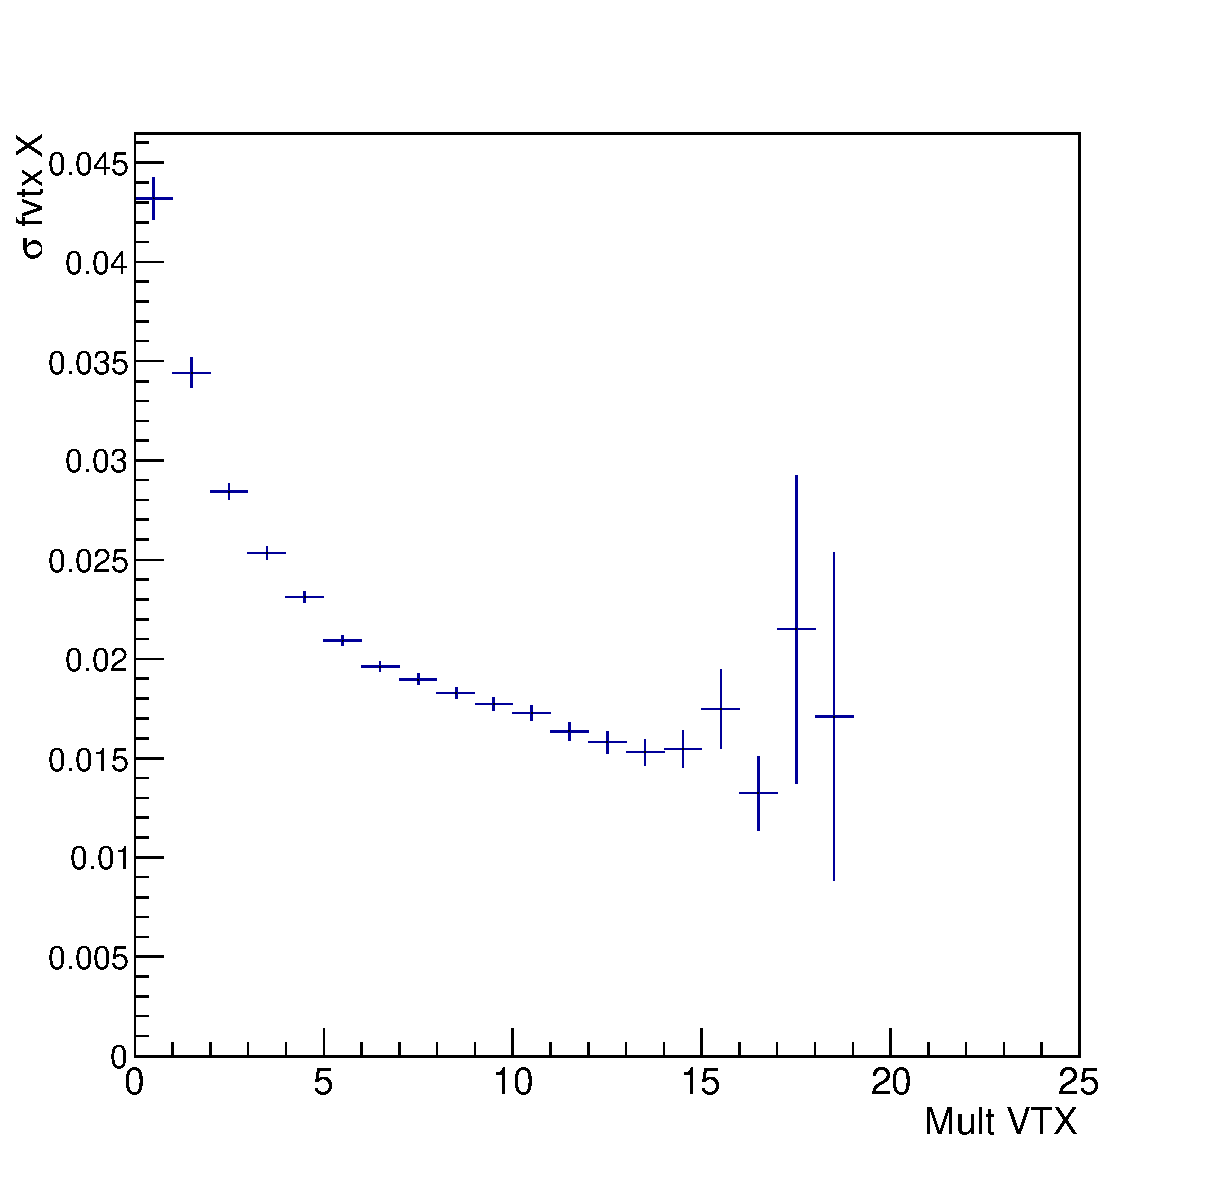
\includegraphics{Figures/fvtxX_v_MultSVX_fit}}} 
\subfigure[]{\resizebox{7cm}{!}{ 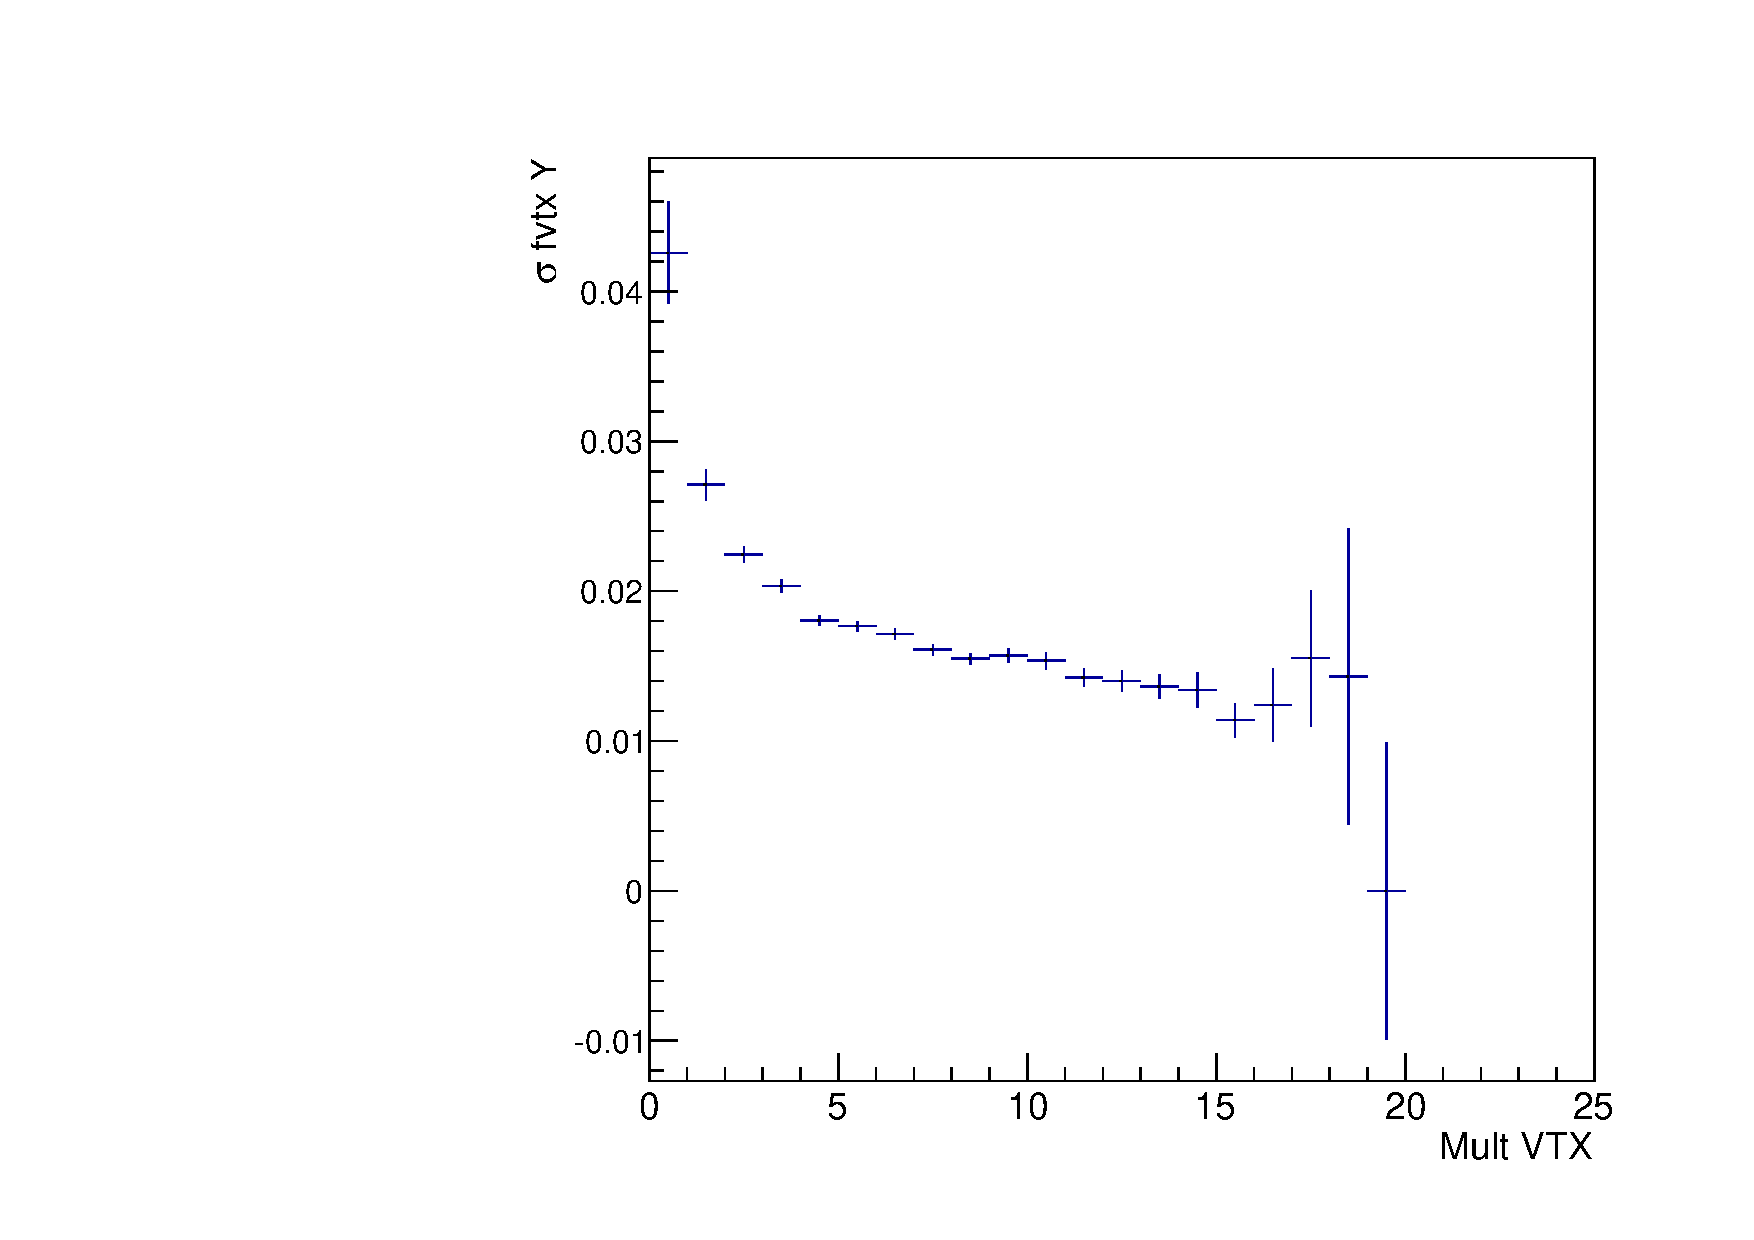
\includegraphics{Figures/fvtxY_v_MultSVX_fit}}} \\
  \caption{Vertex resolution for X (left) and Y (right) versus VTX multiplicity in Run 12 p-p data.}
  \label{fig:DCAResVTXMult}
\end{center}
\end{figure}  


\begin{figure}[t!]
\begin{center}
\subfigure[]{\resizebox{7cm}{!}{ 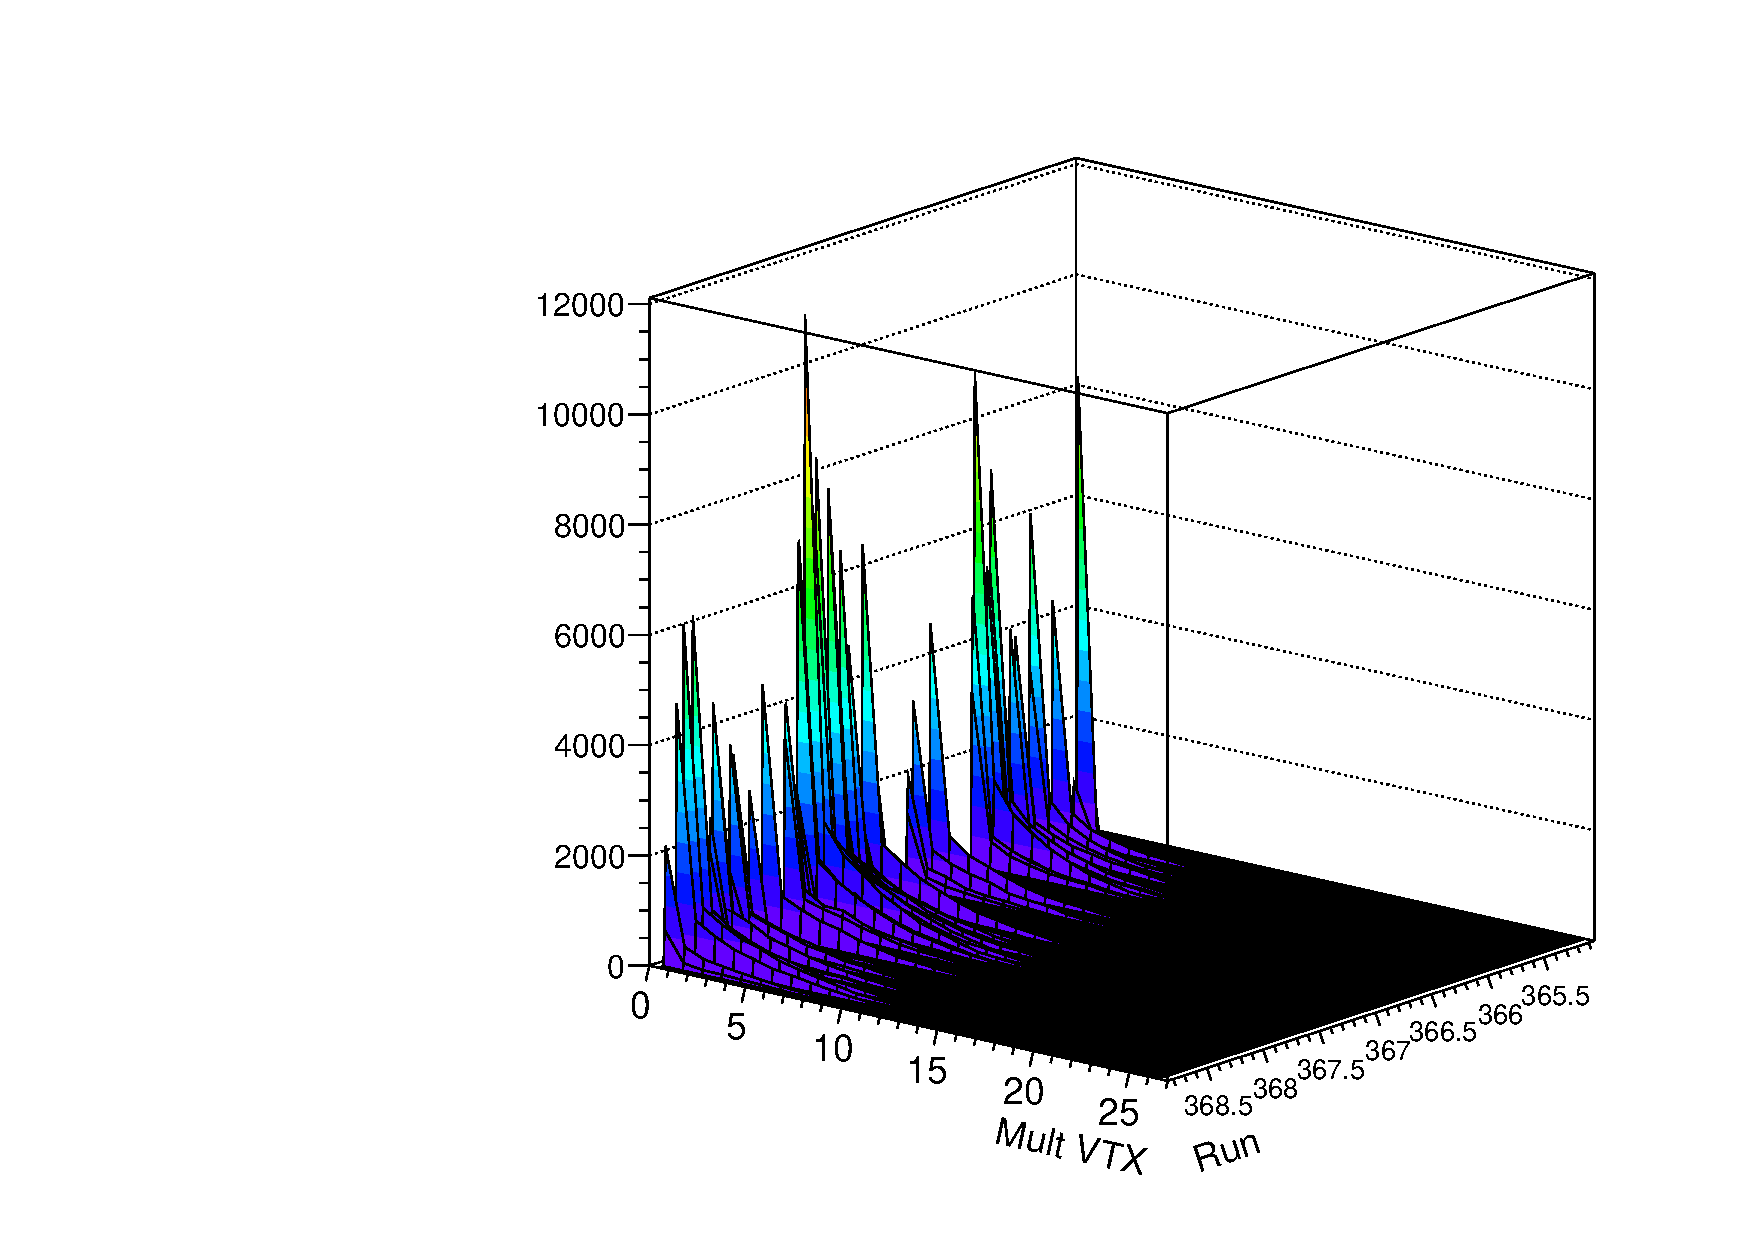
\includegraphics{Figures/MultSVX_v_Run_3D}}} 
\subfigure[]{\resizebox{7cm}{!}{ 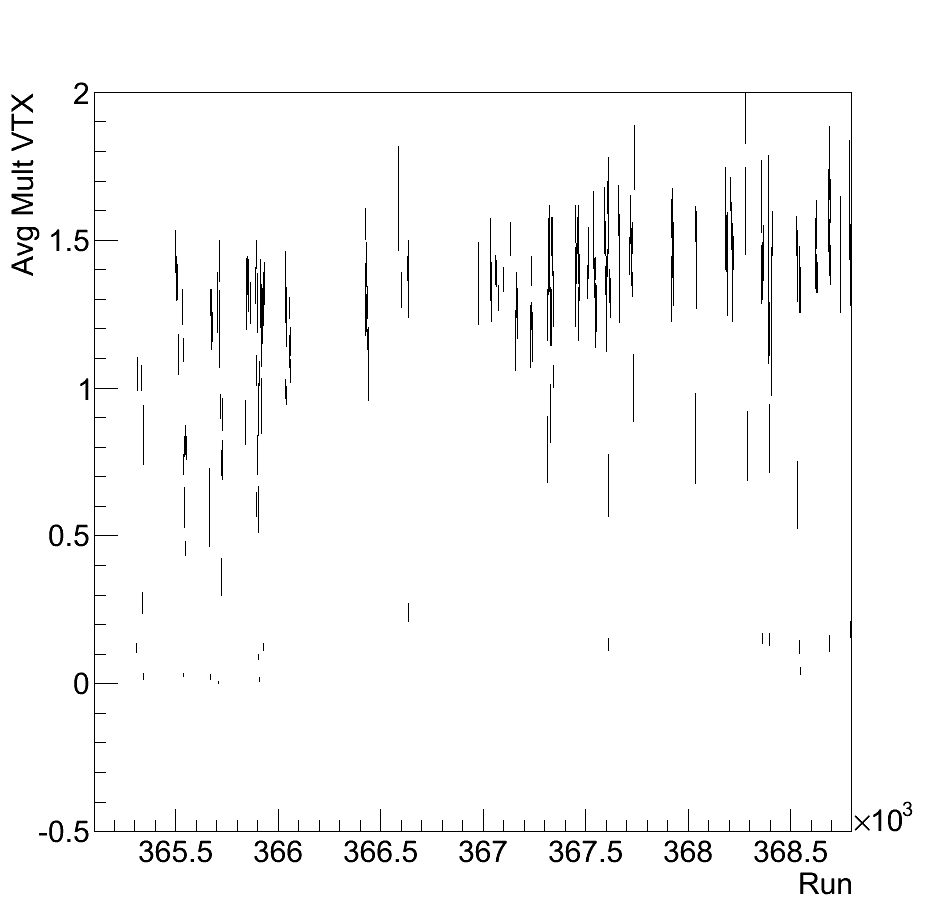
\includegraphics{Figures/AvgMultVTX_v_Run}}} \\
  \caption{Multiplicity in the VTX versus run (left) and average multiplicity in the VTX versus run (right) for all runs in Run 12 p-p data.}
  \label{fig:VTXMult}
\end{center}
\end{figure}  



\begin{figure}[t!]
\begin{center}
\subfigure[]{\resizebox{14cm}{!}{ 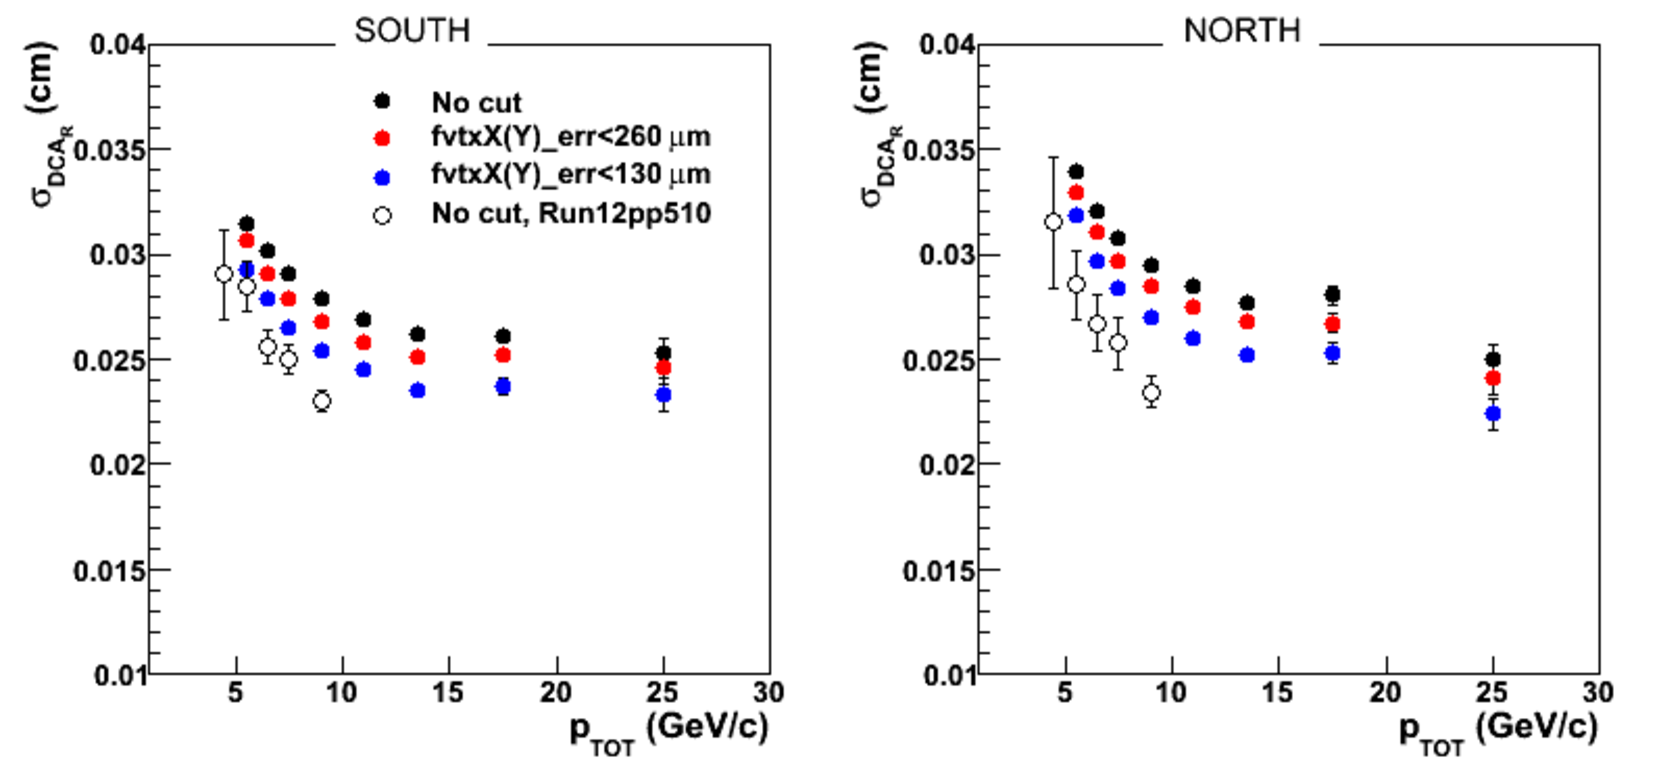
\includegraphics{Figures/Run15pp200_DCAR_sigma_p_before_beam_center}}} 
\subfigure[]{\resizebox{14cm}{!}{ 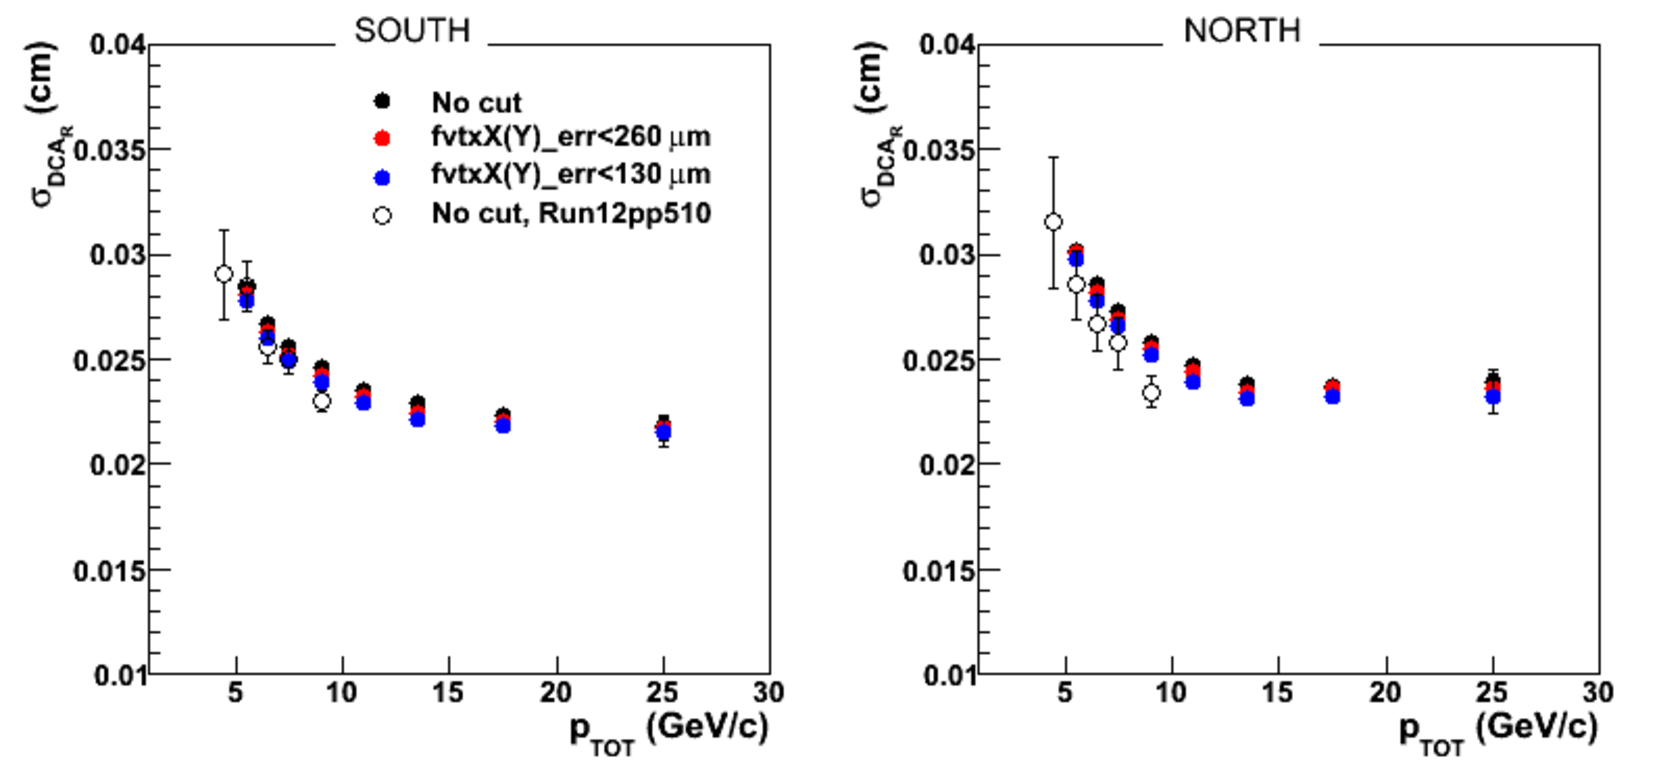
\includegraphics{Figures/Run15pp200_DCAR_sigma_p_after_beam_center}}} \\
  \caption{\dcar resolution before (top) and after (bottom) applying the run-by-run XY beam center.}
  \label{fig:VTXBeamCenter}
\end{center}
\end{figure}  



\newpage

%%%%%%%%%%%%%%%%%%%%%%%%%%%%%%%%%%%%%%%%%%%%%%%%%%%%%%%%%%%%
\section{Data Analysis}
\label{sec:DataAnalysis}

{\color{red}FIXME}
{\color{red}Add good and bad runs}

\subsection{CVS location of the codes and macros}
\label{sec:CVS}

{\color{red}FIXME}

%%%%%%%%%%%%%%%%%%%%%%%%
\subsection{General Procedure}
The goal of this analysis is to measure a B production ratio from the fitting of the \dcar distributions
in data using the \dcar distributions from Monte Carlo.  In this section, the steps for obtaining this measurement are described.
The first step is to select dimuon pairs according to the single muon track selection and dimuon pair cuts that lie within the 
\jpsi mass range and have at least one good match to an FVTX track. This selection will contain \jpsi decays, combinatorial background 
and a continuum background which is much smaller than the combinatorial background.

A dimuon pair can have one or two of its tracks matching FVTX. At the same time, a single muon can match one or 
more FVTX tracklets as long the match and FVTX tracklet quality comply with the requirements defined in Tables \ref{tab:cuts} and \ref{tab:fiducial_cuts}.
 An FVTX-MuTr single muon can be present in several dimuon and FVTX-MuTr match combinations in one event which may introduce double counting.
 A \textit{set} container is used to check if the single muon was already used to fill the histogram in order to prevent double counting.

The \dcar distribution may contain the dimuon combinatorial background (dimuons which are not from \jpsi decays), as well as FVTX-MuTr mismatch 
background (muons from \jpsi which is associated to the wrong FVTX track). The mismatch background is obtained from FVTX-MuTr associations 
where FVTX tracks and MuTr tracks are from different events. In order to reproduce the same event conditions, both events in the mix needs to be 
at the same centrality and Z-vertx category. One hundred Z-vertex and 10 FVTX track multiplicity event categories are used to do this event mixing. 
The mismatch background shape is extracted from prompt hadrons in data in order to gain enough statistics for a smooth shape, while the normalization 
is determined by the frequency of mismatches for muons coming from \jpsi.

A sample of prompt \jpsi and B $\to$ \jpsi decays are produced using \pythia 8 and the detector interaction is simulated with Geant 4. 
These MC samples are tuned to match conditions in Run 12 pp data as close as possible (see Sec. \ref{sec:MCTuning}).  These MC samples 
are used to predict detector resolution and line shape of the \dcar for B $\to$ \jpsi and \jpsi.

The combinatorial background, event swapped FVTX-MuTr match, prompt \jpsi and B $\to$ \jpsi models are fit to the raw \dcar distribution using a
maximum likelihood fit and cross checked with multiple fits to verify statistical errors accuracy. The remainder of this section describes these steps in detail.

%%%%%%%%%%%%%%%%%%%%%%%%
\subsection{Monte Carlo Tuning}
\label{sec:MCTuning}

%\begin{figure}[h]
%\begin{center}
%\includegraphics[width=0.7\textwidth,angle=0]{figures/}
%\\ \caption{}
%\label{fig:MCDataVertexRes}
%\end{center}
%\end{figure}

The simulation and reconstruction of \pythia \jpsi events alone is not enough to accurately reflect the multiplicity or the resolution of
both the vertex and the DCA from data.  First, the multiplicity of the Monte Carlo is increased by throwing not only the \jpsi hard scattering event,
but also a minimum bias event at the same vertex position as the \jpsi hard scattering event.  To keep as much correlation as possible between these
two \pythia events, the minimum bias event is required to have a renormalization scale (Q) approximately the same as the \jpsi event it is being thrown 
with.  In real data, these are one event, however it is clear that \pythia does not get the multiplicity from the soft scattering and underlying event correct 
with the hard scattering event alone. 

%put additional subsubsection (Sanghoon) 
%Approximately 20\% of events in the Run 12 pp 510 GeV data have multiple collision vertices.  To account for this,
%20\% of the \jpsi events contain a second vertex. Figure \ref{fig:SecondaryVtx} shows the differences in X, Y, and Z between the primary vertex and the 
%secondary vertex in data (left) and simulation (right) for events with two or more vertices. 
%A comparison of the track multiplicity in data Monte Carlo is shown in figure \ref{fig:EventMultiplicity}.  


%\begin{figure}[h]
%\begin{center}
%\includegraphics[width=0.7\textwidth,angle=0]{figures/}
%\\ \caption{}
%\label{fig:SecondaryVtx}
%\end{center}
%\end{figure}


%\begin{figure}[h]
%\begin{center}
%\includegraphics[width=0.7\textwidth,angle=0]{figures/}
%\\ \caption{}
%\label{fig:EventMultiplicity}
%\end{center}
%\end{figure}


Once the multiplicity reflects that of data, noise is added to the muon tracking to reflect more accurately the noise in the real detector. 
This has little effect on the resolution, as it will mostly just decrease the quality of tracks by making more tracks that contain
some random noise hits and fewer hits overall than good tracks.  Because this effect is negligible to the \dcar resolution and introduces
a large amount of time to the Monte Carlo creation, we do not introduce extra noise into our full Monte Carlo samples.  

Next, the best known dead channel masking is applied to the Monte Carlo to capture the efficiency loss and extra effects these dead areas may introduce.
A large fraction (63\%) of the useable Run 12 pp dataset has a dead or nearly dead VTX.  This has a large effect on the resolution
of the vertex as shown in figure \ref{fig:DCA_v_VTX}.  Because the \dcar resolution is dominated by vertex resolution for tracks above 3 GeV,
the vertex resolution becomes the most important part of the \dcar resolution for most of our signal events.  

To make the Monte Carlo  accurately reflect this inefficiency in the Run 12 pp dataset, a random run selection of dead maps is introduced.  
When producing the Monte Carlo, a random run detector setup is picked according to the fraction of total luminosity collected in that run.  
The full simulation is then performed on that run for that job.  This is repeated across a large set of statistics so as to repeat the detector 
setup across the full Run 12 pp dataset. Figure \ref{fig:DCAFromJPsi_Tuned} (left) shows the DCA distribution from simulated \jpsi events 
after these tuning steps as compared with selected \jpsi events from data (right). 
%%%%%%%%%%%%%%%%%%%%%%%%%%%%%%%%%%%%%%%%%%%%%%%%%%%%%%%%
\subsubsection{Multiple collisions}
Because of high luminosity duing 510 GeV pp run, there are some chances of multiple collisions in a single MB event. 
For pp runs, FVTX vertex reconstruction module for tagging additional primary vertices is utilized.
Figure~\ref{fig:FvtxZ_2nd} shows fraction of events including 2nd vertex to events of \fvtxz is within $\pm10~{\rm cm}$ as a function of BBC rate (left) and difference of \fvtxz between 1st and 2nd vertices. 

\begin{figure}[!h]
\begin{center}
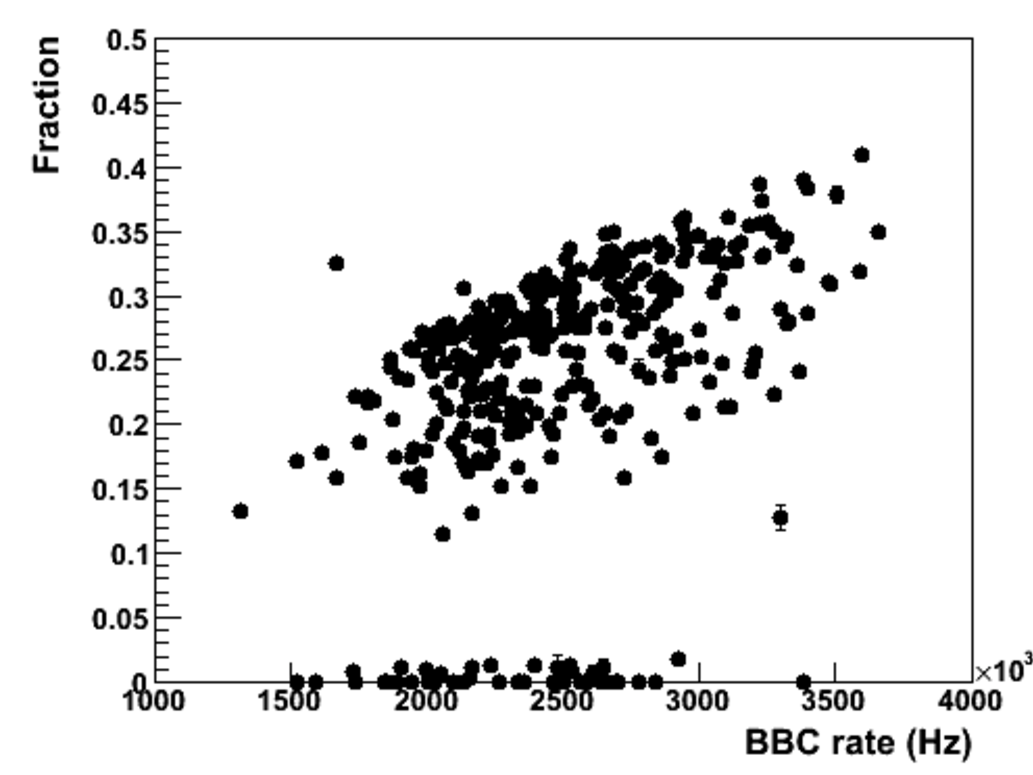
\includegraphics[width=0.5\textwidth,angle=0]{figures/Fraction_2nd_vertex_BBCrate}
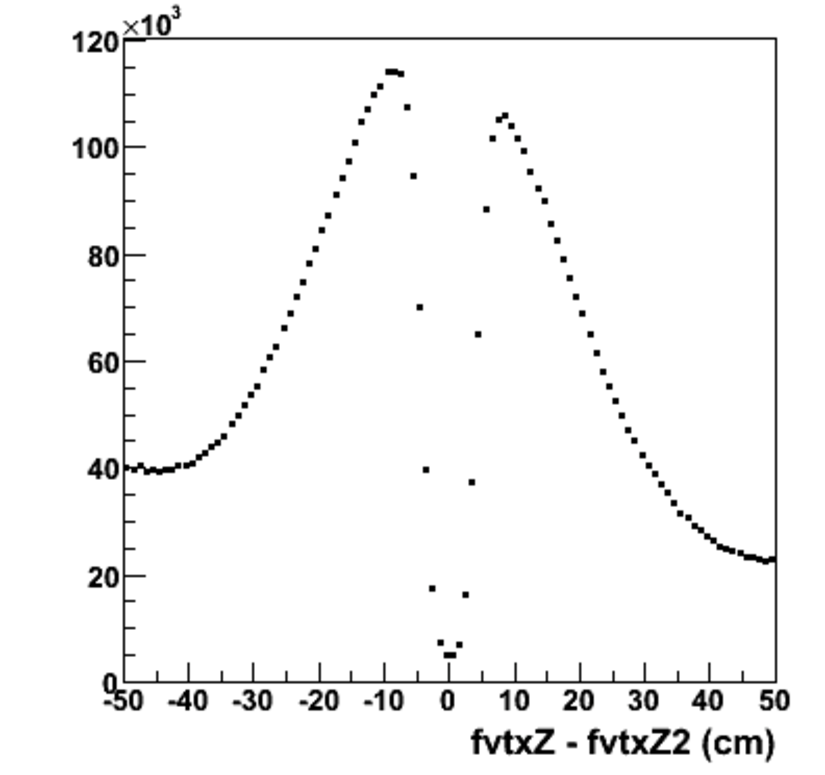
\includegraphics[width=0.4\textwidth,angle=0]{figures/FvtxZ_diff_1st_2nd}
\\ \caption{Fraction of events having two reconstructed vertices (left) and the distribution of difference between two \fvtxz.}
\label{fig:FvtxZ_2nd}
\end{center}
\end{figure}


The fraction of events including 2nd primary vertex is increasing as BBC rate goes high.
Assuming there is no correlation between two collisions in a single beam crossing, the probability to successfully reconstruct 2nd vertex drops dramatically when location of two collisions is close ($<10~{\rm cm}$) as shown in the right plot of figure~\ref{fig:FvtxZ_2nd}.
In this case, the reconstructed \fvtxz could be in between real positions of two collisions, and this would affect \dcar distributions.
In order to deal with this problem, we also perform 2 vertices simulation, which introduce additional minimum bias event at random location, and combine with 1 vertex simulation.
Figure~\ref{fig:dca_1vtx_2vtx} shows \dcar distributions of \jpsi simulation with 1 vertex and 2 vertices (BUT events of only 1 vertex is successfully reconstructed) at South (left) and North (right).
There is a clear enhancement at large \dcar in case of two collisions are happend closely.

\begin{figure}[!h]
\begin{center}
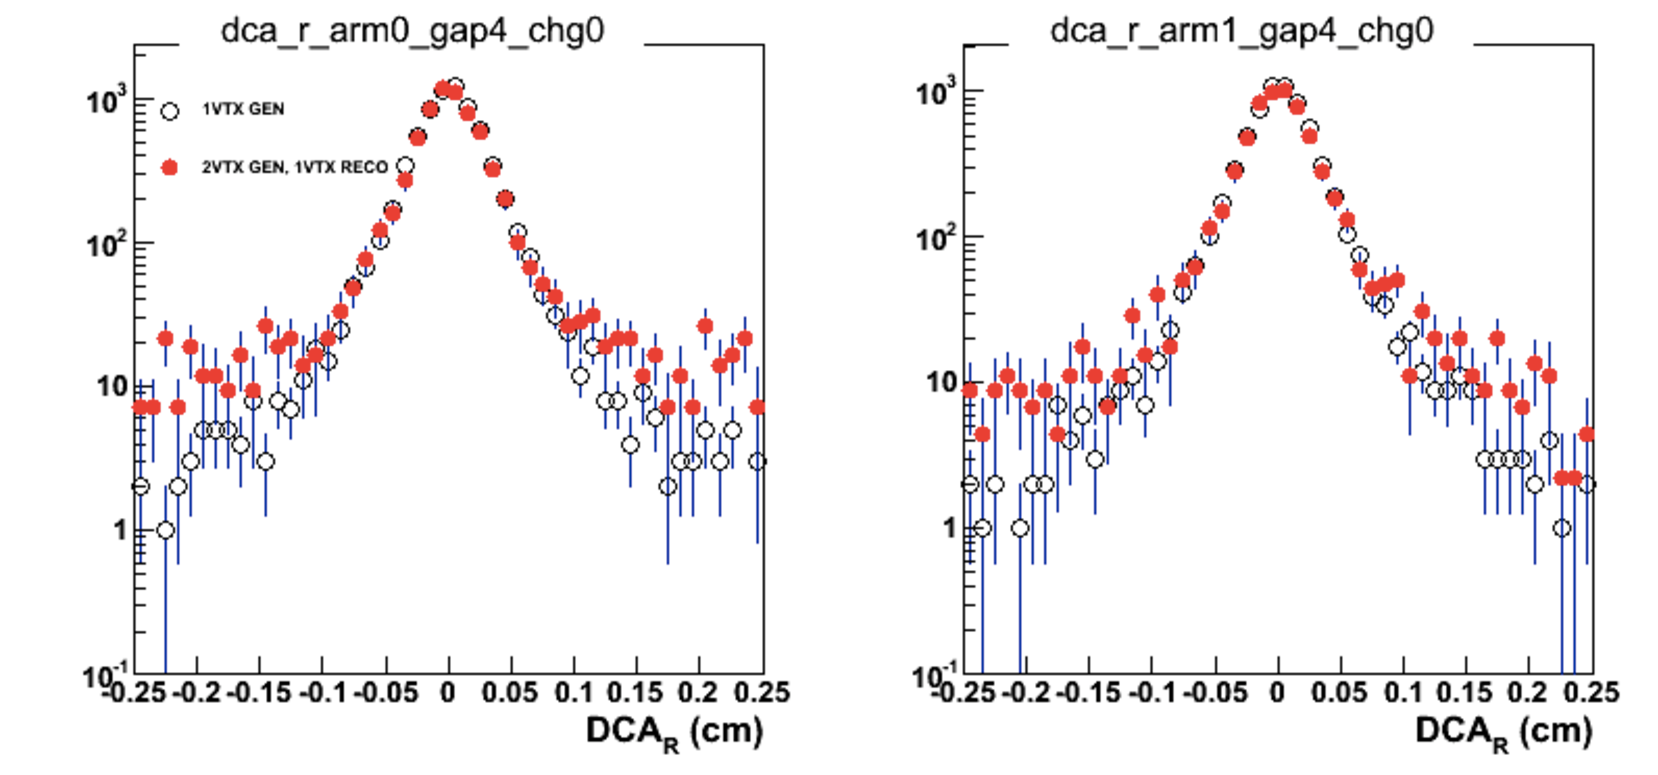
\includegraphics[width=0.8\textwidth,angle=0]{figures/dca_r_1vtx_2vtx_1miss}
\\ \caption{Comparion of \dcar distribution between \jpsi simulations with 1 vertex or 2 vertices (select only 1 vertex is reconstructed) at South (left) and North (right) arms.}
\label{fig:dca_1vtx_2vtx}
\end{center}
\end{figure}

\begin{figure}[!h]
\begin{center}
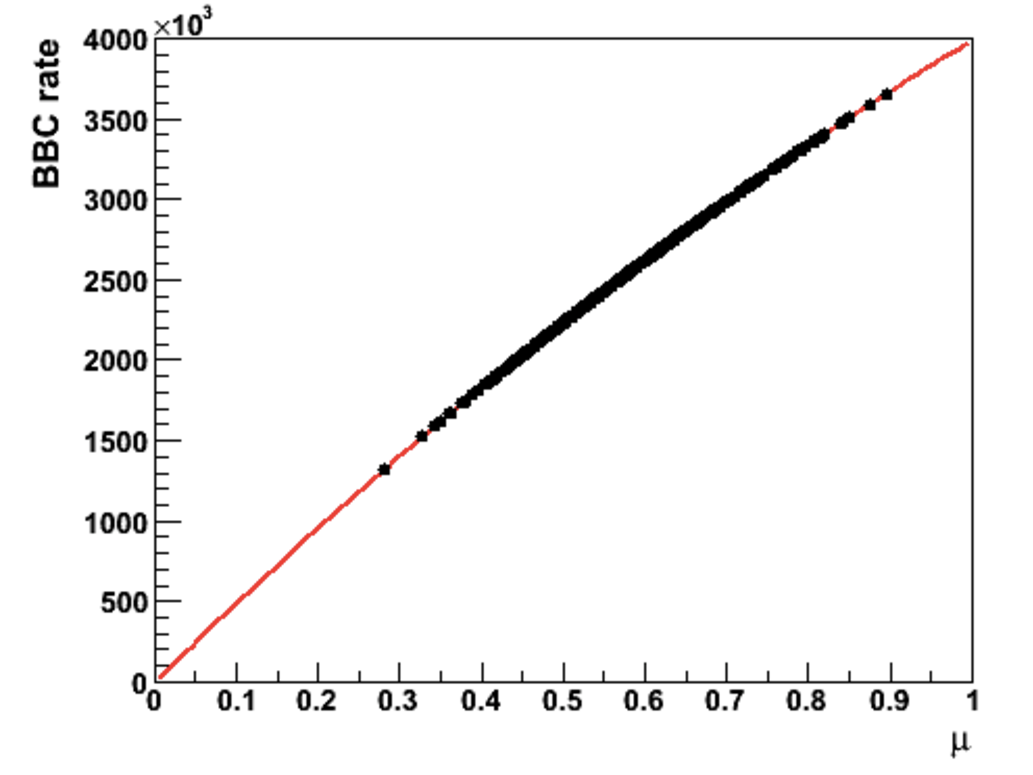
\includegraphics[width=0.4\textwidth,angle=0]{figures/multi_collision_par_BBC_rate}
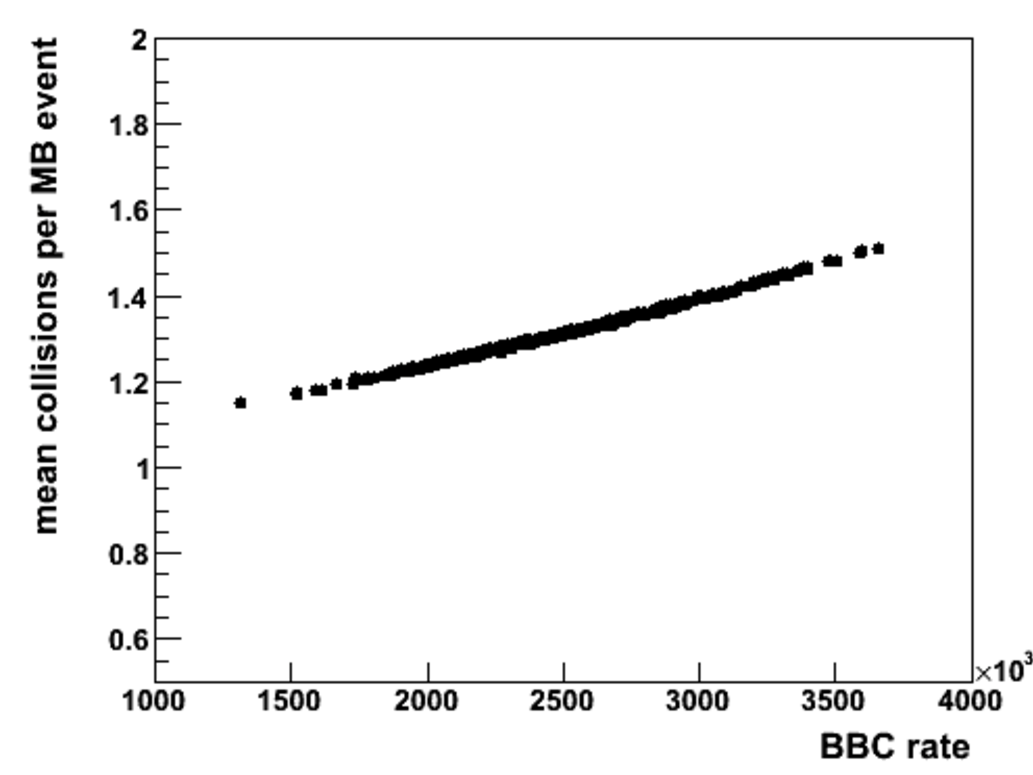
\includegraphics[width=0.4\textwidth,angle=0]{figures/mean_collision_per_BBC_rate}
\\ \caption{Relation between multiple collision parameter ($\mu$) and BBC rate (left) and estimated number of mean collisions (right).}
\label{fig:multi_collision}
\end{center}
\end{figure}

In order to combine two simulations with correct ratio, we follow the estimation method from previous study for $W$ analysis~\cite{ref:an1103}. Based on the relation between multiple collision parameter ($\mu$) and BBC rates presented in the left plot of figure~\ref{fig:multi_collision}, we calculate the number of mean collisions per minimum bias event (at least one collision) for each BBC rate of Run12 pp run as shown in the right plot of figure~\ref{fig:multi_collision}. By taking account the fraction of collisions within $\pm20~{\rm cm}$ (36.3\%) from the $Z_{\rm BBC}$ distribution of low BBC rate runs and integrated luminosity for each run in Run12 pp, we estimate 11.68\% of 2 collisions events, both events are in $|Z|<20~{\rm cm}$ which is consistent with the simulation setup, in the entire Run12 pp minimum bias events.


%%%%%%%%%%%%%%%%%%%%%%%%%%%%%%%%%%%%%%%%%%%%%%%%%%%%%%%%
%\begin{figure}[h]
%\begin{center}
%\includegraphics[width=0.7\textwidth,angle=0]{figures/}
%\\ \caption{}
%\label{fig:DCA_v_VTX_Frac}
%\end{center}
%\end{figure}

%\begin{figure}[h]
%\begin{center}
%\includegraphics[width=0.7\textwidth,angle=0]{figures/}
%\\ \caption{}
%\label{fig:DCA_v_VTX}
%\end{center}
%\end{figure}


%%% Might need this as well...
%Even with all the previous tuning steps, there is still some disagreement with simulated events.
%The simulated vertex can be smeared during reconstruction in the X, Y, Z directions to account for this extra resolution seen in data.
%Figure \ref{fig:DCAFromJPsi_Tuned_Smeared} shows the DCA distribution from simulated \jpsi events after all previous tuning and with this
%extra vertex smearing.
%%%

%\begin{figure}[h]
%\begin{center}
%\includegraphics[width=0.7\textwidth,angle=0]{figures/}
%\\ \caption{}
%\label{fig:DCAFromJPsi_Tuned}
%\end{center}
%\end{figure}

%\begin{figure}[h]
%\begin{center}
%\includegraphics[width=0.7\textwidth,angle=0]{figures/}
%\\ \caption{}
%\label{fig:DCAFromJPsi_Tuned_Smeared}
%\end{center}
%\end{figure}

%%%%%%%%%%%%%%%%%%%%%%%%%%%%%%%%%%%%%%%%%%%%%%%%%%%%%%%%
\subsection{Selection}

%%%%%%%%%%%%%%%%%%%%%%%%
\subsubsection{Muon Selection}
\label{sec:selection}

{\color{red} THIS NEEDS TO BE FINALIZED}
A summary of all cuts applied for single muons and dimuons is listed in Table \ref{tab:cuts}.

\begin{table}[!hb]
		\caption{\label{tab:cuts} List of all single muon and dimuon cuts applied in this analysis.}
	    \begin{tabular}{llcc}
    	& & south & north\\\hline
    	\multirow{17}{*} {Single Muon cuts} 
	& MuID last gap & $=$ 4 & $=$ 4 \\
    	& N hits in MuID & $\ge$ 6 & $\ge$ 6 \\
    	& DG0*p & $<$ 80 & $<$ 80 \\
    	& DDG0*p & $<$ 40 & $<$ 40 \\
    	& MuTr-MuID match $\chi^2$ & $<$ 3 & $<$ 3 \\
    	& MuTr track $\chi^2$ & $<$ 10 & $<$ 10 \\
    	& N hits in MuTr & $>$ 11 & $>$ 11 \\
    	& $p_Z$ & $>$ 3 GeV/c & $>$ 3 GeV/c \\
    	& N hits in FVTX track & $>$ 2 & $>$ 2 \\
    	& FVTX+MuTr matching $\chi^2$ (Sec. \ref{sec:matching})& $<$ 5 & $<$ 5 \\
%    	& azimuthal residual at FVTX st4 (Sec.\ref{sec:matching}) & $<$0.1 & $<$0.1 \\
        & Radial residual at FVTX st4 $\le$ &  9.1-1.7p+0.11$\rm{p}^{2}$ & 8.1-1.4p+0.09$\rm{p}^{2}$ \\
        & Azimuthal residual at FVTX st4 $\le$ &  0.4-0.08p+0.006$\rm{p}^{2}$ & 0.4-0.07p+0.005$\rm{p}^{2}$ \\
        & Polar residual at FVTX st4 $\le$ &  0.2-0.03p+0.002$\rm{p}^{2}$ & 0.2-0.04p+0.002$\rm{p}^{2}$ \\
%    	\multicolumn{3}{c}{fiducial cuts (Sec.\ref{sec:fiducial cuts})} \\  	
   	& $\textrm{DCA}_{\phi}$ (3$\sigma$ cut) & \multicolumn{2}{c}{$<$ 3$\cdot$(0.6-0.05p+0.0015p$^{2}$) } \\ 
   	& \multicolumn{3}{l}{Track should project to the same FVTX primary vertex }\\
   	& (either FVTX or FVTX\_SECOND) \\ 	
	\hline
    	\multirow{2}{*}{Dimuon cuts} 
	& Vertex projection $\chi^2$ & $<$ 3  & $<$ 3 \\
%    	& \multicolumn{3}{l}{muon pair should not share same MuTr octant}\\
%    	& asymmetry = $\frac{p1 - p2}{p1 + p2}$ & $<$ 0.6 & $<$ 0.6 \\
    	& 2.7 $<$ mass\footnote{as determined by MuTr track only} GeV/$\rm{c}^{2}$ $<$ 3.5 \\\hline
    	\multirow{2}{*}{Event cuts} 
	& $|\textrm{FVTX Z vertex}|$ &   \multicolumn{2}{c}{$<$ 10 cm} \\
    	& FVTX Z vertex error      &   \multicolumn{2}{c}{ $<$ 400 $\mu$m} \\\hline
    \end{tabular}
\end{table}

\pagebreak
\newpage


%%%%%%%%%%%%%%%%%%%%%%%%
\subsubsection{Dimuon Selection}
\label{sec:dimuon_selection}

The Mutr-MuID matching parameters are:

\begin{description}
	\item [DG0:] is the distance between the MuTr track and MuID road projections at the MuID gap containing a hit closest to the vertex
	\item [DDG0:] is the angle between the MuTr track and MuID road
	\item [idchi2:] is the $\chi^2$ of the matching considering the projections at all MuID gaps
\end{description}

The MuTr-MuID matching parameters DG0 and DDG0 have a strong dependence with the
momentum of the single muon as seen in Figure \ref{fig:DG0_cut}. A cut on DG0$\times$momentum 
showed to be more appropriated to account for the momentum dependence of DG0. A similar procedure is applied for DDG0 cut used for the MuTr-MuID matching.
 
Each muon in an event is associated with an event vertex. For this analysis, both muons 
in the dimuon pair are required to match the same primary
vertex determined from the FVTX. This cut becomes important since the FVTX
primary vertex works as a point to fit the dimuon. There is no DCA cut in this selection since the
projections using only the MuTr can be on the order of few cm. 
The vertex projection $\chi^2$ is obtained from a fit of the dimuon tracks with the vertex. 

%%%%%%%%%%%%%%%%%%%%%%%%
\subsection{Primary Vertex Determination}
\label{sec:PVDet}

MIKE

%%%%%%%%%%%%%%%%%%%%%%%%%%%%%%%%%%%%%%%%%%%%%%%%%%%%%%%%
\subsection{FVTX-MuTr Combined Track Calculation and Projection to the Primary Vertex}
\label{sec:combine_fvtx_mutr}

Each FVTX-MuTr match forms a combined track which is used to extract the momentum, the track vertex and its DCAs. 
The vertex should be on a plane perpendicular to the Z-axis and placed at the Z-vertex determined from the primary vertex finder. 
The FVTX track and the MuTr track are projected to this plane returning their corresponding momentum and vertex vectors.
The calculation uses as input an array $\hat{Y}$ containing the momentum and vertex projection vectors from FVTX and MuTr. 
The combined result $\hat{A}$ is related to the input by the correlation matrix $\hat{X}$ 

\begin{equation}
\overbrace{\left(\begin{array}{c}x_{mutr}\\y_{mutr}\\px_{mutr}\\py_{mutr}\\pz_{mutr}\\x_{fvtx}\\y_{fvtx}\\px_{fvtx}\\py_{fvtx}\\pz_{fvtx}\\ Evt\_fvtxX\\ Evt\_fvtxY\end{array}\right)}^{\hat{Y}} 
= \overbrace{\left(\begin{array}{ccccc}1&0&0&0&0\\ 0&1&0&0&0\\ 0&0&1&0&0\\ 0&0&0&1&0\\ 0&0&0&0&1\\1&0&0&0&0\\ 0&1&0&0&0\\ 0&0&1&0&0\\ 0&0&0&1&0\\ 0&0&0&0&1\\1&0&0&0&0\\0&1&0&0&0  \end{array}\right)}^{\hat{X}}
\cdot \overbrace{\left(\begin{array}{c} x0\\ y0 \\ px \\ py \\ pz \end{array} \right)}^{\hat{A}}.
\end{equation}

The 5$\times$5 covariant matrices from MuTr ($cov_{mutr}$), FVTX ($cov_{fvtx}$) projections and vertex determination $(cov_{Evt_fvtx})$ are accommodated in the matrix $\hat{V}$

\begin{equation}
\hat{V} = \left(\begin{array}{ccc} cov_{mutr} & 0 & 0\\ 0 & cov_{fvtx} & 0 \\ 0 & 0 & cov_{Evt\_fvtx} \end{array} \right).
\end{equation}

The combined FVTX-MuTr track momentum and vertex array $\hat{A}$ is thus obtained from the matrix equation
\begin{equation}
	\hat{A} = \left(\hat{X}^t \hat{V}^{-1} \hat{X}\right)^{-1} \hat{X}^t \hat{V}^{-1}\hat{Y}
\end{equation}

%%%%%%%%%%%%%%%%%%%%%%%%%%%%%%%%%%%%%%%%%%%%%%%%%%%%%%%%
\subsection{FVTX-MuTr mismatch determination}
\label{sec:mismatch}

\begin{figure}
\begin{center}
\subfigure[]{\resizebox{8cm}{!}{	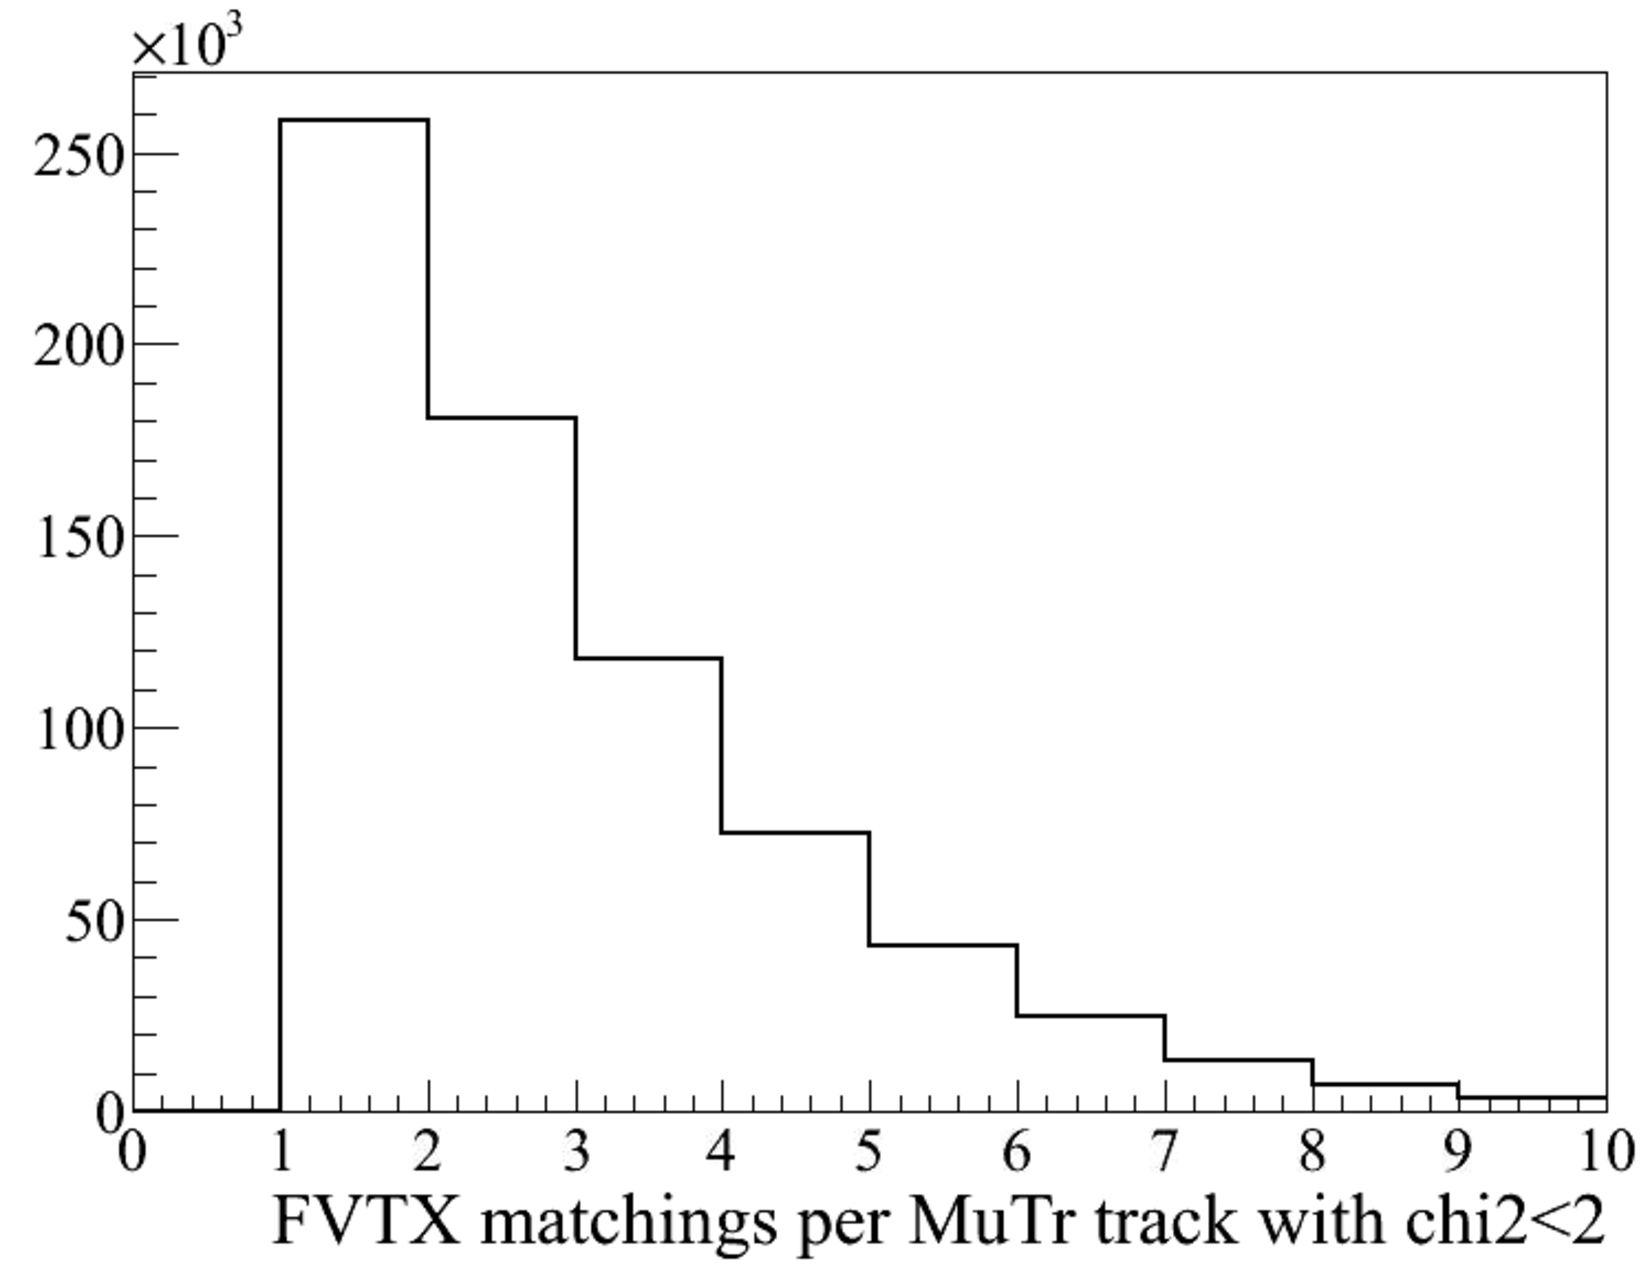
\includegraphics[width=0.45\textwidth]{Figures/n_matchings} } }
\subfigure[]{\resizebox{12cm}{!}{
	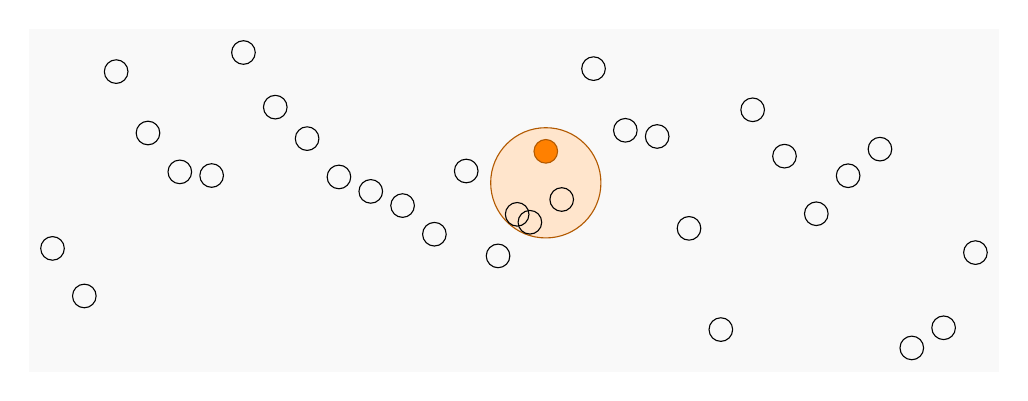
\begin{tikzpicture}
	[background rectangle/.style={fill=gray!5!white,draw=white},show background rectangle]
		
	\filldraw[fill=orange!20!white, draw=orange!70!black] (0.55\textwidth, 0.1) circle (.7);
		
	\filldraw[fill=orange, draw=orange!70!black] (0.55\textwidth, 0.5) circle (.15);
	\draw (0.52\textwidth, -0.3) circle (.15);
	
	\foreach \i in {1,2,...,30}
	\draw (\textwidth*\i/30, rand*2.0) circle (.15);
	\end{tikzpicture}
}}
	\caption{\label{fig:mismatch}(a)Distribution of the number of FVTX-MuTr matches per MuTr track. (b)Schematic view of the multiple matchings.}
\end{center}
\end{figure}

The last FVTX plane and the first MuTr station are 150 cm apart and have 1m of absorber material in between. A MuTr track projection at FVTX station 4 forms 
a cone with radius up to 2 cm for muons with momentum of 3 GeV, because of the multiple scattering in the absorber. As a result, 64\% of the MuTr projections find 
more than one FVTX track inside its cone projection size (Fig. \ref{fig:mismatch}).

\begin{figure}[!htb]
	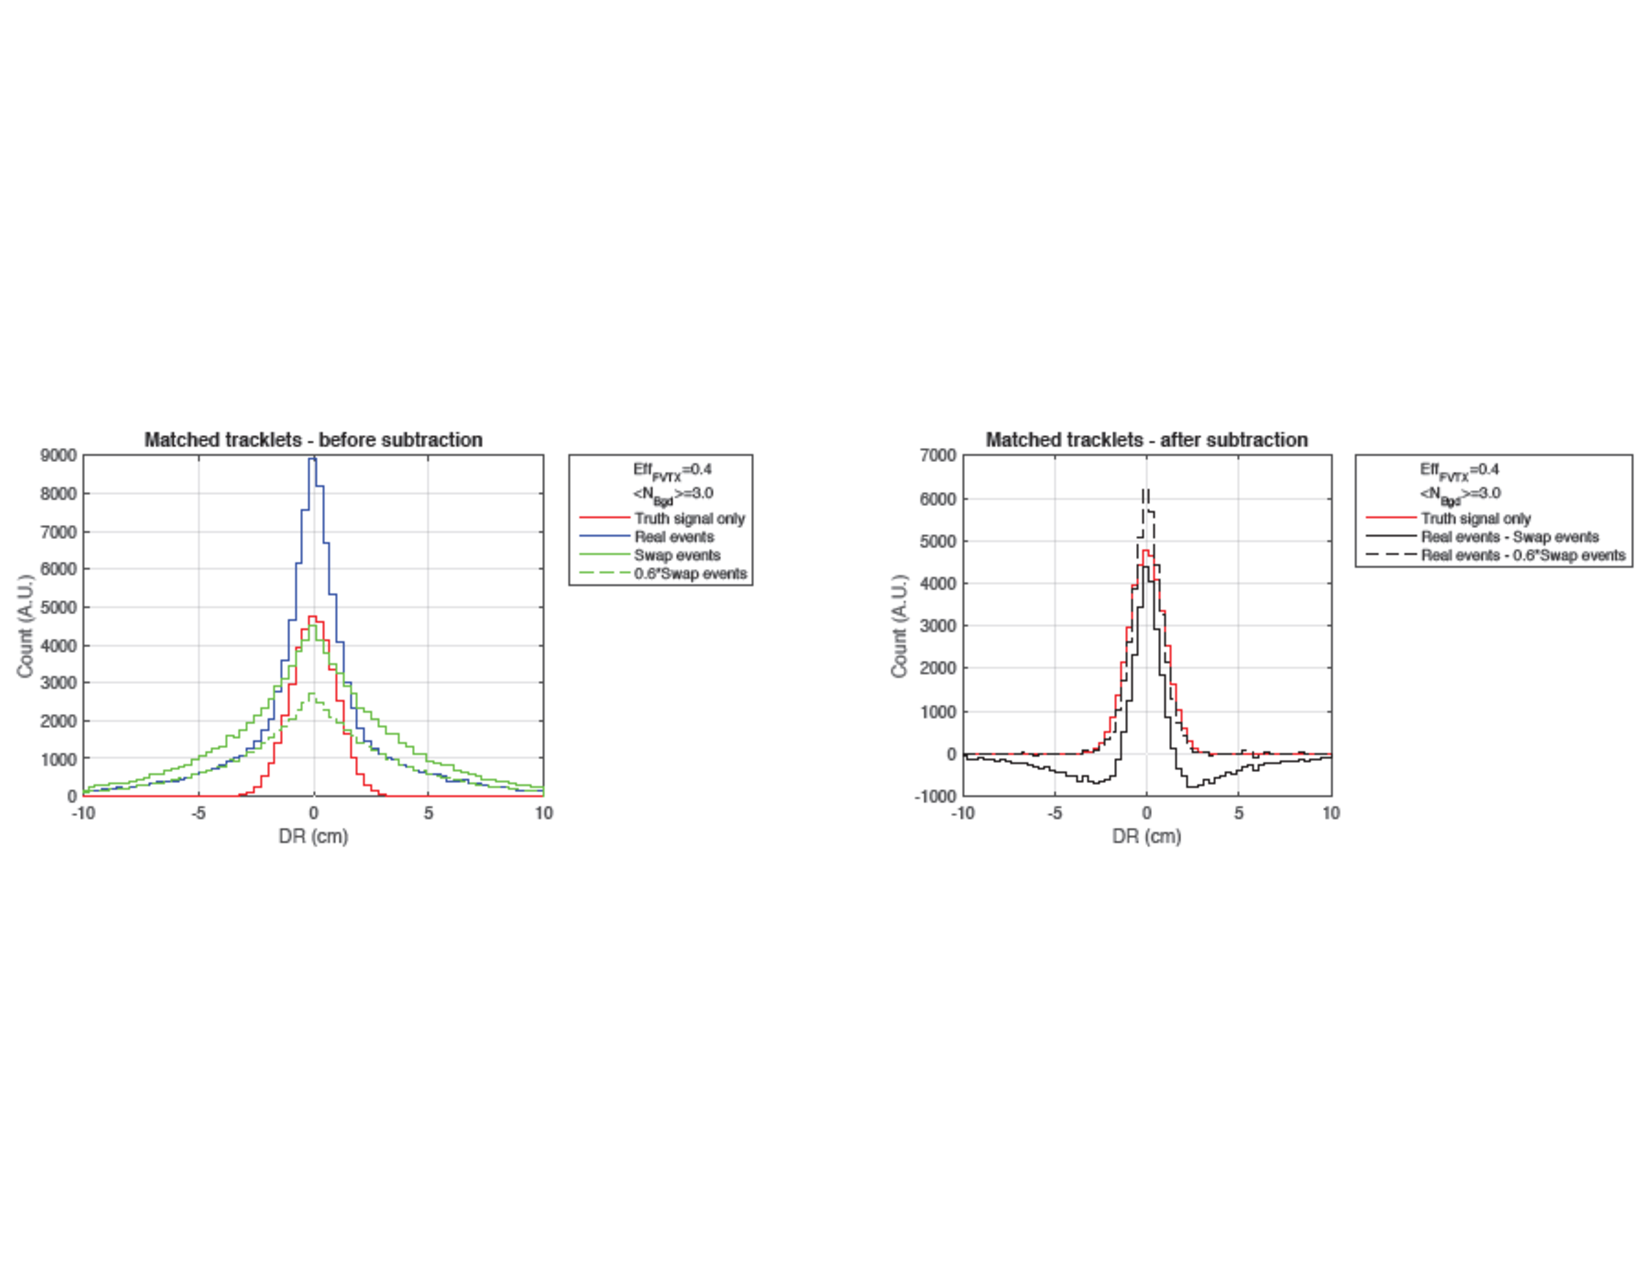
\includegraphics[width=1.0\textwidth]{Figures/swapp_bias}	
	\caption{\label{fig:toy_model_match} General residual distribution from a Toy Monte Carlo study in the presence of multiple possible associated matches. 
	(left) Results for the raw residual distribution, event swapped distribution and the truth residual. 
	(right) Comparison between the true residual and the event swapped distribution when only the best match is chosen.}
\end{figure}

Using the best FVTX-MuTr association based on matching $\chi^2$ (\ref{eq:match_chi2}) is statistically incorrect. There is no guarantee 
that the best $\chi^2$ is the right match if there are 2 or more associations satisfying the match $\chi^2<3$ condition. 
The other problem in choosing only a best match is a bias in the $\chi^2$ and \dcar distribution. The best $\chi^2$ match 
residual distribution is not the same as the distribution of a true match $\chi^2$. A toy Monte Carlo study using a simple ideal detector 
showed that once a best matching is required in a distribution and any mismatch subtraction is used, the residuals will be biased not only 
 the normalization, but also in the shape of the residual distributions (Fig. \ref{fig:toy_model_match}-a). Indeed, when a best match is required, 
 the \dcar distribution after mismatch subtraction from mixed events shows a small negative counts at \dcar$\sim$0.2.

\begin{figure}[!htb]
	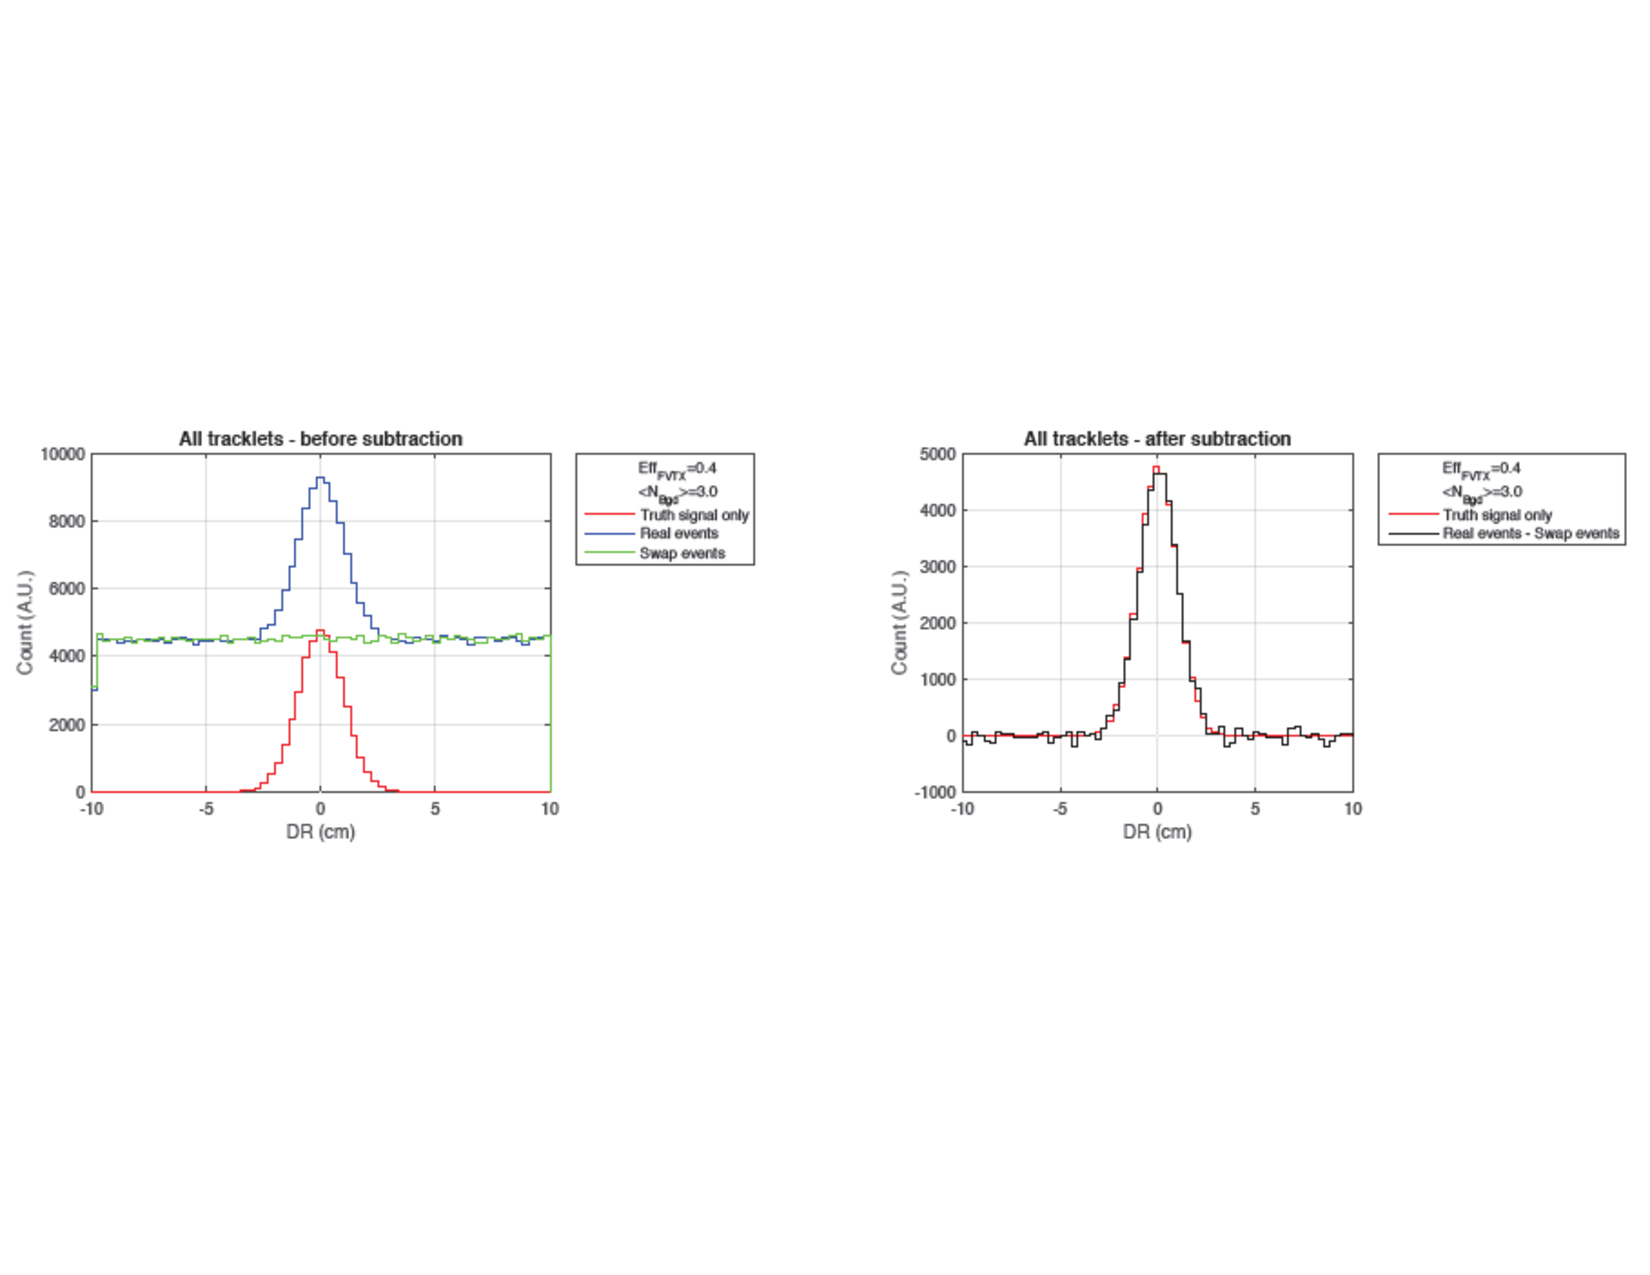
\includegraphics[width=1.0\textwidth]{Figures/swapp_bias_combinatorics}
	\caption{\label{fig:toy_model_match_nobias} (left) Residual distribution from a Toy Model where all matching combinations are kept. (right)Residual after event mixed match subtraction.}
\end{figure}

The solution for the problem mentioned above is to keep all FVTX-MuTr track matchings. The same Toy Models studies showed that if there is 
no best match requirement, there is no bias either in the normalization nor the shape of the residuals (Fig. \ref{fig:toy_model_match_nobias}).

True residual and \dcar distributions are obtained from all matchings after an uncorrelated mismatch distribution. The uncorrelated match is 
obtained by matching MuTr and FVTX tracks from different events. To be as realistic as possible, the mixed events needs to belong to the same 
centrality (for Heavy Ion) and Z-vertex category. The maximum size of the centrality and Z-vertex bins were evaluated in order to not introduce 
any bias to the \dcar distribution. This study was performed with embedded simulation where different bin sizes were experimented and the \dcar 
distribution were compared with the ones from identified Monte Carlo tracks. Despite the large projection uncertainty of the MuTr, Z-vertex bins 
larger than 2mm started to show some bias in the \dcar distributions. In the case of Heavy Ions, centrality is categorized by a more direct 
measurement: the FVTX track multiplicity. Using 10\% track multiplicity bins did not affected \dcar distributions. 


In summary, all  FVTX-MuTr tracks obeying the cuts defined in Tables \ref{tab:cuts} and \ref{tab:fiducial_cuts} are accepted. Random match combinations 
are obtained in event mixed FVTX-MuTr matchings within 2mm Z-vertex bins.

Despite the normalization of the event mixed FVTX-MuTr match being unbiased, a non-unity normalization still is necessary to account for events in the beginning 
of the processing job which does not find a former event at the same category. The way to account for this effect and any possible centrality bias is to count the
 total number of tracks in the event $N_{\rm tracks}$ and the total number of tracks in swapped events $N_{\rm stracks}$. The ratio of the total track counts

\begin{equation}
\label{eq:swap_norm}
   \textrm{swap normalization} = \frac{N_{\rm tracks}}{N_{\rm stracks}}
\end{equation}

\noindent accounts for the relative track density of the sample analyzed. This normalization ranges between 1.02 to 1.05 depending on how long is the processing 
job and sample used,  triggered data usually producing larger normalization corrections. The mismatch subtraction was tested in several distributions in embed simulation. A description of these tests is found is Section \ref{sec:mismatch_mc}.

{\color{red} NEED TO PUT SWAP DISTRIBUTION FROM PP510}

\pagebreak
\newpage


%%%%%%%%%%%%%%%%%%%%%%%%%%%%%%%%%%%%%%%%%%%%%%%%%%%%%%%%
\subsection{Post-production alignment}
\label{sec:postprod_alignment}

The FVTX alignment procedure uses all FVTX tracklets available in zero field runs. There is no quality check on these tracks nor a matching requirement to MuTr tracks. 
The alignment using Milippede allows offsets in a limited degrees of freedom.

Detector offsets of a few tens of microns may not affect the measurement of the detector resolution which is on the order of 150 to 200 $\mu$m, 
but can introduce artificial tails in \dcar distribution biasing the B-meson decay measurement. 

\begin{figure}
\begin{center}
	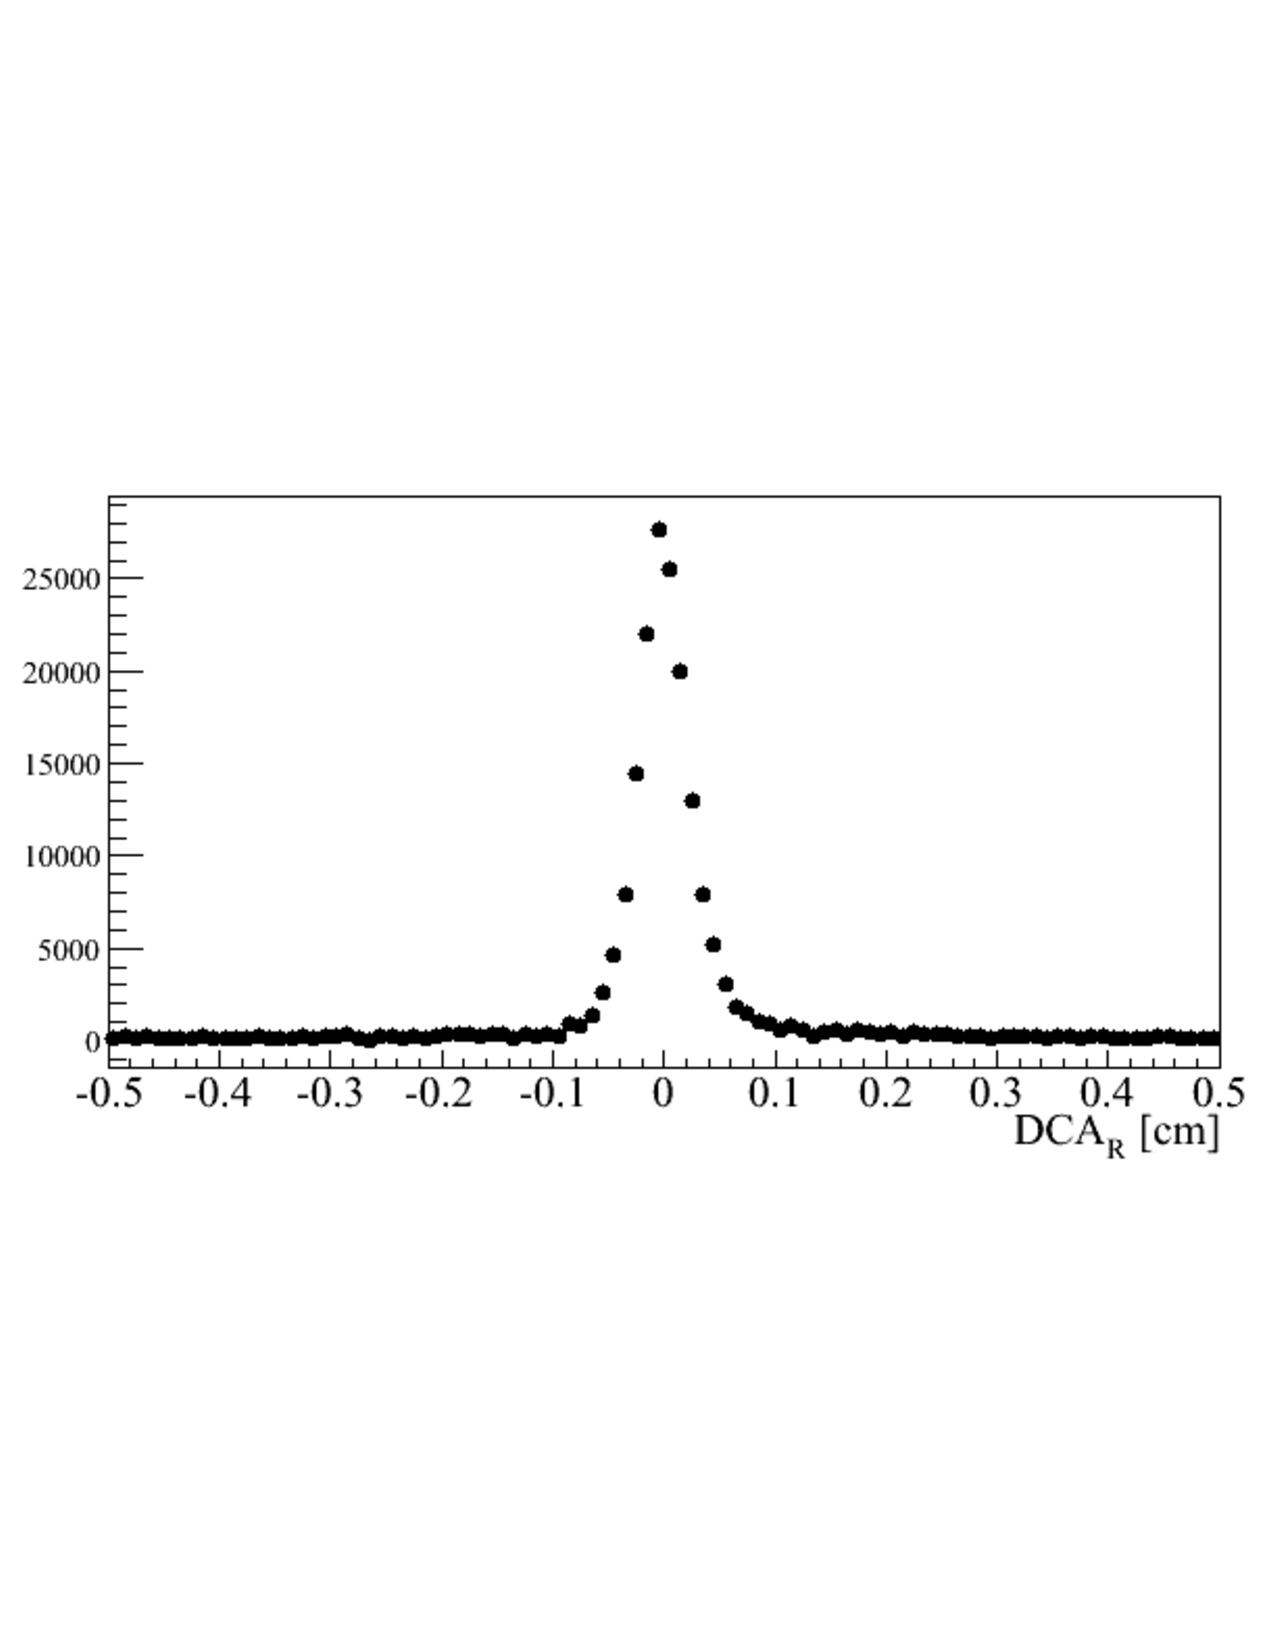
\includegraphics[width=0.5\textwidth]{Figures/dca_hadrons}
	\caption{\label{fig:dca_hadrons}\dcar distribution of stopped hadrons used for FVTX alignment. {\color{red} REPLACE ME}}
\end{center}
\end{figure}

A verification of the FVTX alignment with VTX and hence the primary vertex was performed using tracks which shows MuID activity in the second and third gap, but 
not in gap four. The majority of these tracks are from stopped hadrons which are essentially prompt particles. There are nearly {\color{red} XXX} stopped tracks over the Run 12 pp
 data which can be used for an alignment check (Fig. \ref{fig:dca_hadrons}). Events with large vertex error, tracks next to dead areas and bad quality FVTX tracks 
 are removed from this sample.

\begin{figure}
	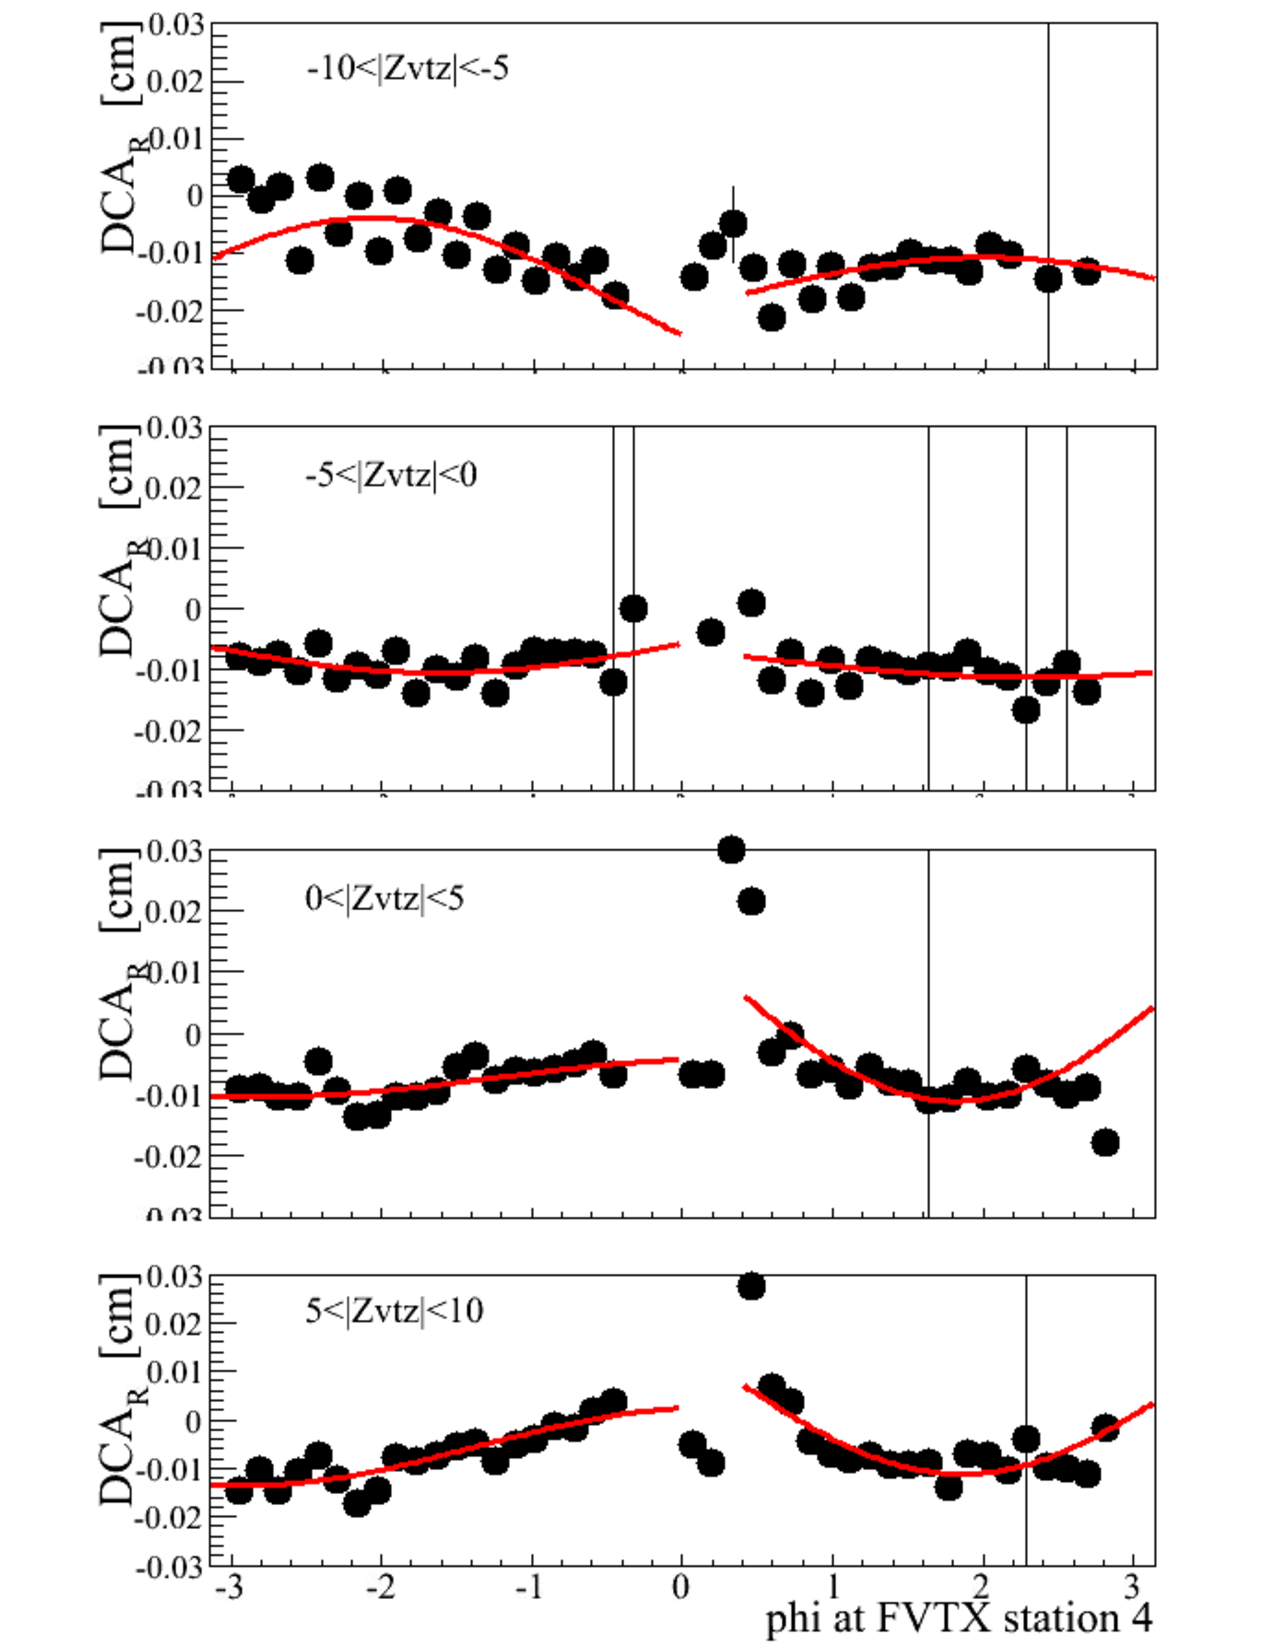
\includegraphics[width=0.49\linewidth]{Figures/dcar_phi_z_south}
	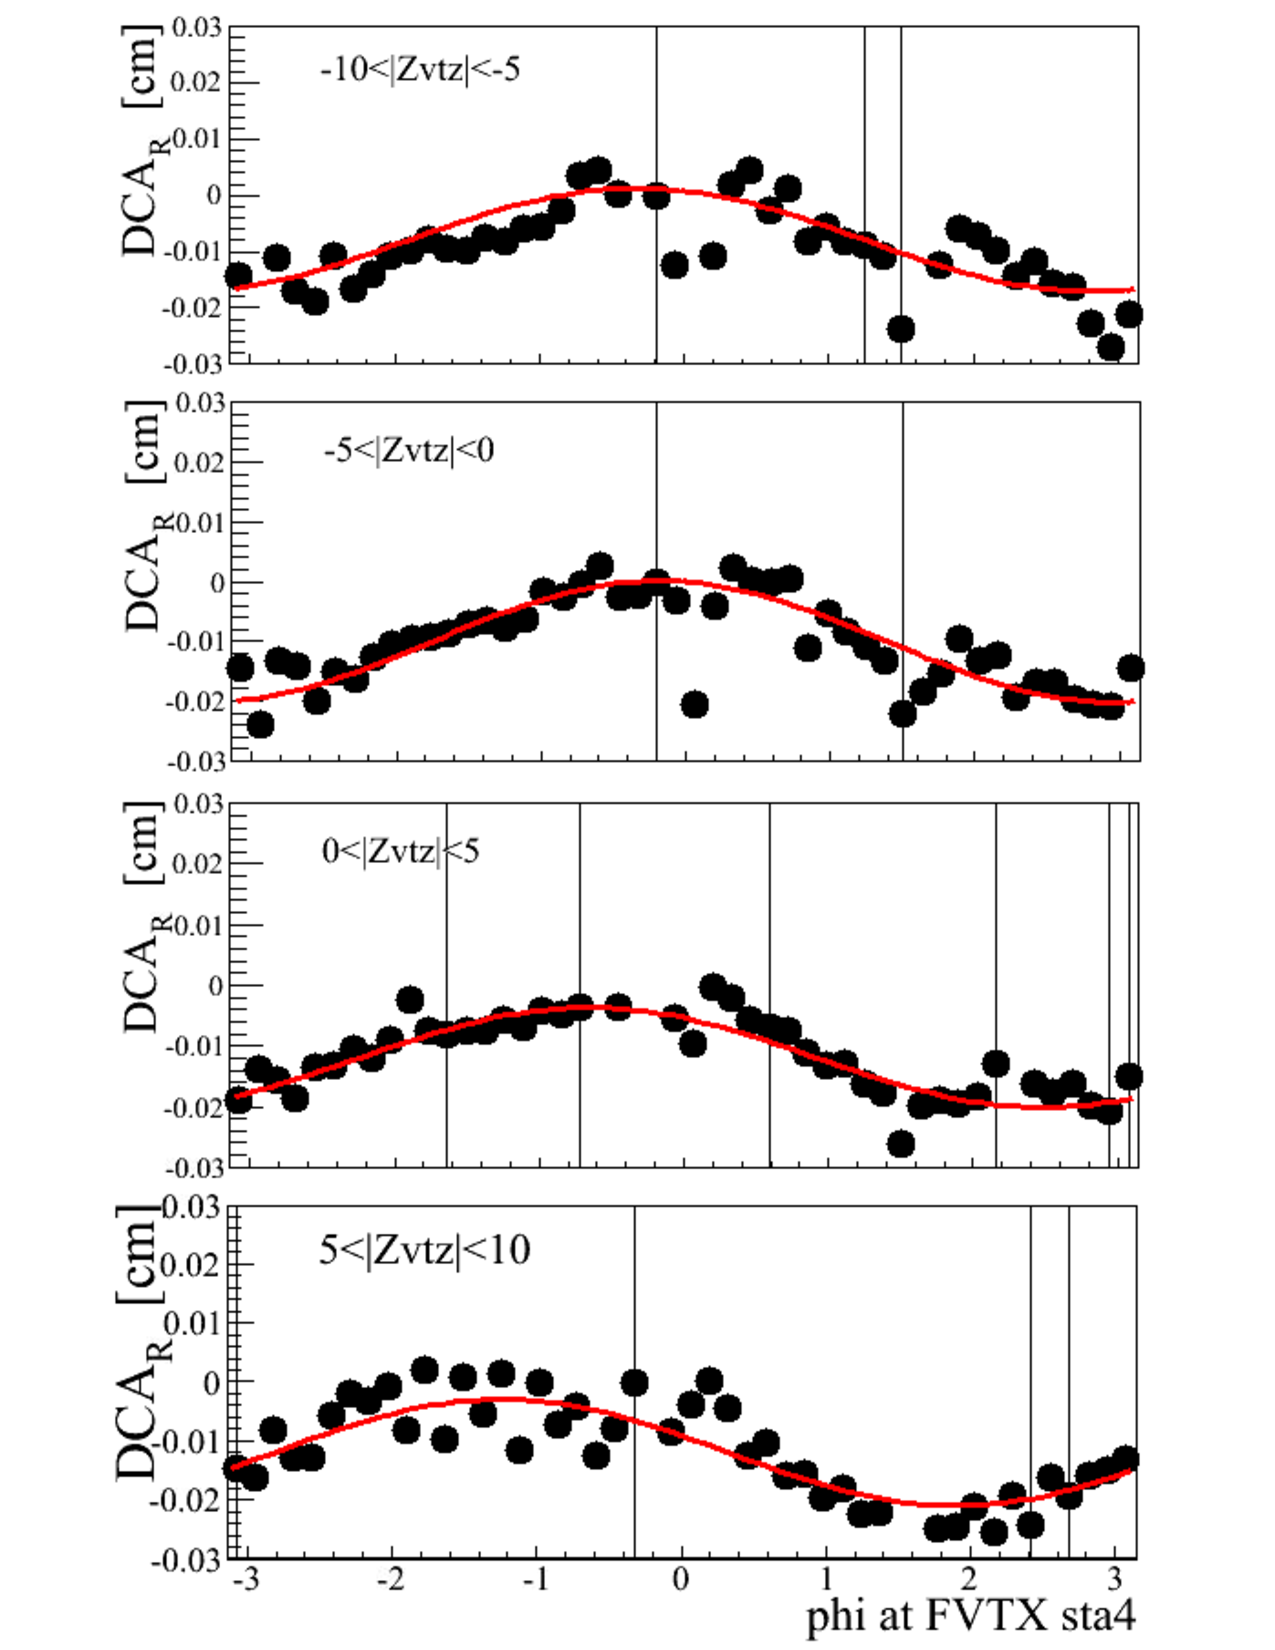
\includegraphics[width=0.49\linewidth]{Figures/dcar_phi_z_north}
	\caption{Azimuthal dependence of \dcar at 4 Z-vertex ranges. The $\phi<0(>0)$ corresponds to the EAST(WEST) FVTX cage.{\color{red} REPLACE ME}}
	\label{fig:dcar_phi_z}
\end{figure}

In the alignment check we are looking for modulations in the \dcar mean value as a function of $\phi$ projection at FVTX station 4. 
The only source of modulation is offsets in the FVTX alignment. Hadron and heavy flavor decays can introduce offsets in \dcar, but not modulations. 
We use combined FVTX+MuTr tracks for this purpose. In a first alignment stage the track cannot have a VTX hit since its presence can bias the alignment. 
Figure \ref{fig:dcar_phi_z} shows the azimuthal dependence of the \dcar centroid in four Z-vertex ranges. The centroids were obtained from a Gaussian 
fit in each $\phi$ bin. Modulations are observed in all cages and their magnitudes change with Z-vertex range. 

The modulations in each Z-vertex bin are described from the $\Delta X$, $\Delta Y$ offsets:

\begin{equation}
\label{eq:dcar_offset}
{\rm DCA}_{\rm uncorr} = \textrm{offset} + \Delta X cos(\phi) + \Delta Y \cdot sin(\phi)
\end{equation}

\begin{figure}
	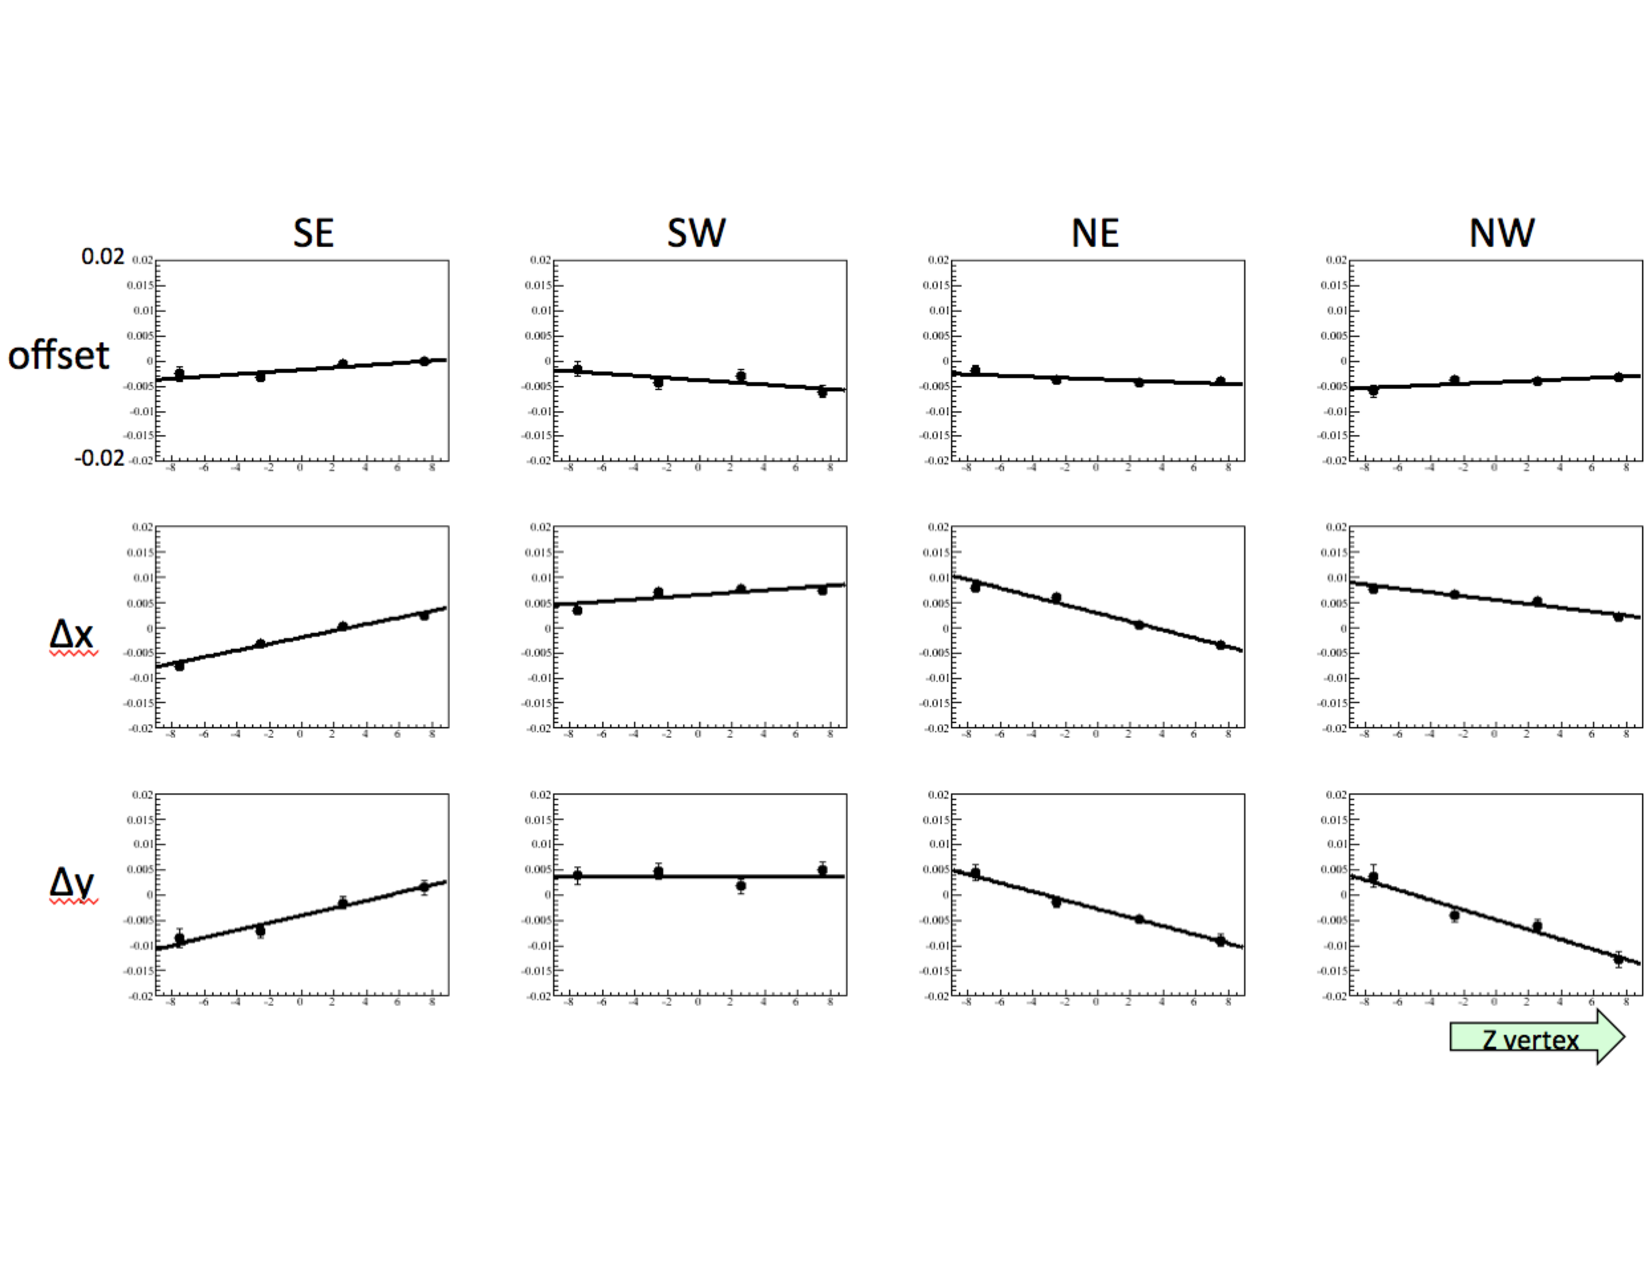
\includegraphics[width=1.0\textwidth]{Figures/alignment_pretiltcorr}
	\caption{\label{fig:fvtx_offsets} Z-vertex dependence of \dcar offsets for each FVTX cage.{\color{red} REPLACE ME}}
\end{figure}

\begin{figure}[!htb]
\subfigure[]{\resizebox{9cm}{!}{
		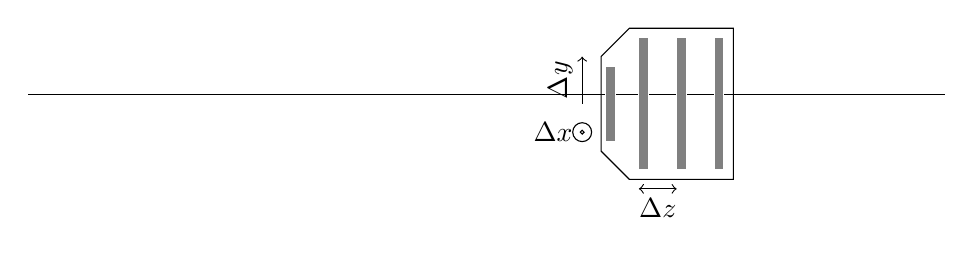
\begin{tikzpicture}[scale=1.2]
		\draw (-0.5\textwidth, 0.1) -- (0.3\textwidth,0.1);
		\filldraw[fill=gray, draw=white]  (0.05, -0.4) rectangle +(0.1,0.8);
		\filldraw[fill=gray, draw=white]  (0.4,-0.7) rectangle +(0.1,1.4);
		\filldraw[fill=gray, draw=white]  (0.8,-0.7) rectangle +(0.1,1.4);
		\filldraw[fill=gray, draw=white]  (1.2,-0.7) rectangle +(0.1,1.4);
		\draw (0,0) -- (0, 0.5) -- (0.3,0.8) -- (1.4,0.8) -- (1.4,-0.8) -- (0.3,-0.8) -- (0,-0.5) -- (0,0);
		\draw[->] (-0.2,0) -- node[sloped,above,midway] {$\Delta y$} (-0.2,0.5);
		\draw (-0.2,-0.3) circle (0.02);
		\draw (-0.2,-0.3) circle (0.1) node[left] {$\Delta x$};
		\draw[<->] (0.4,-0.9) -- node[below]{$\Delta z$} (0.8,-0.9);
		\end{tikzpicture}	
%		\subcaption{Offset degrees of freedom}
}}
\subfigure[]{\resizebox{9cm}{!}{
		
\begin{tikzpicture}[scale=1.2]
		\draw (-0.3\textwidth, 0) -- (0.5\textwidth,0);
		\filldraw[fill=gray, draw=white,rotate=10]  (0.05, -0.4) rectangle +(0.1,0.8);
		\filldraw[fill=gray, draw=white,rotate=10]  (0.4,-0.7) rectangle +(0.1,1.4);
		\filldraw[fill=gray, draw=white,rotate=10]  (0.8,-0.7) rectangle +(0.1,1.4);
		\filldraw[fill=gray, draw=white,rotate=10]  (1.2,-0.7) rectangle +(0.1,1.4);
		\draw[rotate=10] (0,0) -- (0, 0.5) -- (0.3,0.8) -- (1.4,0.8) -- (1.4,-0.8) -- (0.3,-0.8) -- (0,-0.5) -- (0,0);
		\draw (0,0) -- (0,-1);
		\draw[rotate=10] (0,0) -- (0,-1);
		\draw (0,-0.95) -- node [below] {$\theta_Y$} (0.15,-0.9);
		\end{tikzpicture}
%		\subcaption{Tilt degree of freedom.}	
}}
	\caption{\label{fig:alignment}Degrees of freedom of the FVTX fine tuning alignment.}
\end{figure}

A summary of the offsets obtained from the fitting function (\ref{eq:dcar_offset}) can be seen in Figure \ref{fig:fvtx_offsets}. The offsets show a clear linear 
dependence with the Z-vertex (Fig \ref{fig:alignment}-b)

\begin{eqnarray}
	\Delta X(Z_{\rm vertex}) &=& \Delta X_0 + \frac{dx}{dz} Z_{\rm vertex}\\\nonumber
	\Delta Y(Z_{\rm vertex}) &=& \Delta Y_0 + \frac{dy}{dz} Z_{\rm vertex}
\end{eqnarray}

\noindent where $\Delta X_0$ and $\Delta Y_0$ are cage offsets; $dx/dz$ and $dy/dz$ are FVTX cage tilts (Fig. \ref{fig:alignment}-b) relative to the beam axis. Tilt angles are 

\begin{eqnarray}
\theta_X &=& tan^{-1}\left(\frac{dx}{dz}\right)\\\nonumber
\theta_Y &=& tan^{-1}\left(\frac{dy}{dx}\right)
\end{eqnarray}

All tracks are rotated by $\theta_X$ around the Y-axis and by $\theta_Y$ around the X-axis. Residual modulations from $\Delta X_0$ and $\Delta Y_0$ offsets 
are corrected by shifting the tracks (Fig. \ref{fig:alignment}-a). 

The non-modulated offset term in Eq. (\ref{eq:dcar_offset}) can be caused by decay contributions in the sample or by a Z-axis offset which is not constrained 
during the standard alignment procedure. A real Z-offset of the FVTX cage will also de-focus the track projections causing the \dcar distribution 
width to increase. Based on the last assumption, tracks were shifted in Z-axis by up to 100 $\mu$m.

In the second stage, we verify if there is any additional alignment correction for tracks containing at least one VTX hit. After considering the limited Z-vertex 
acceptance of these tracks, we found VTX hits were introducing an offset of about 50 $\mu$m on north west cage. The final azimuthal dependence 
of the \dcar centroid is shown in Figure \ref{fig:dca_phi_after_alignment}. 

\begin{figure}
	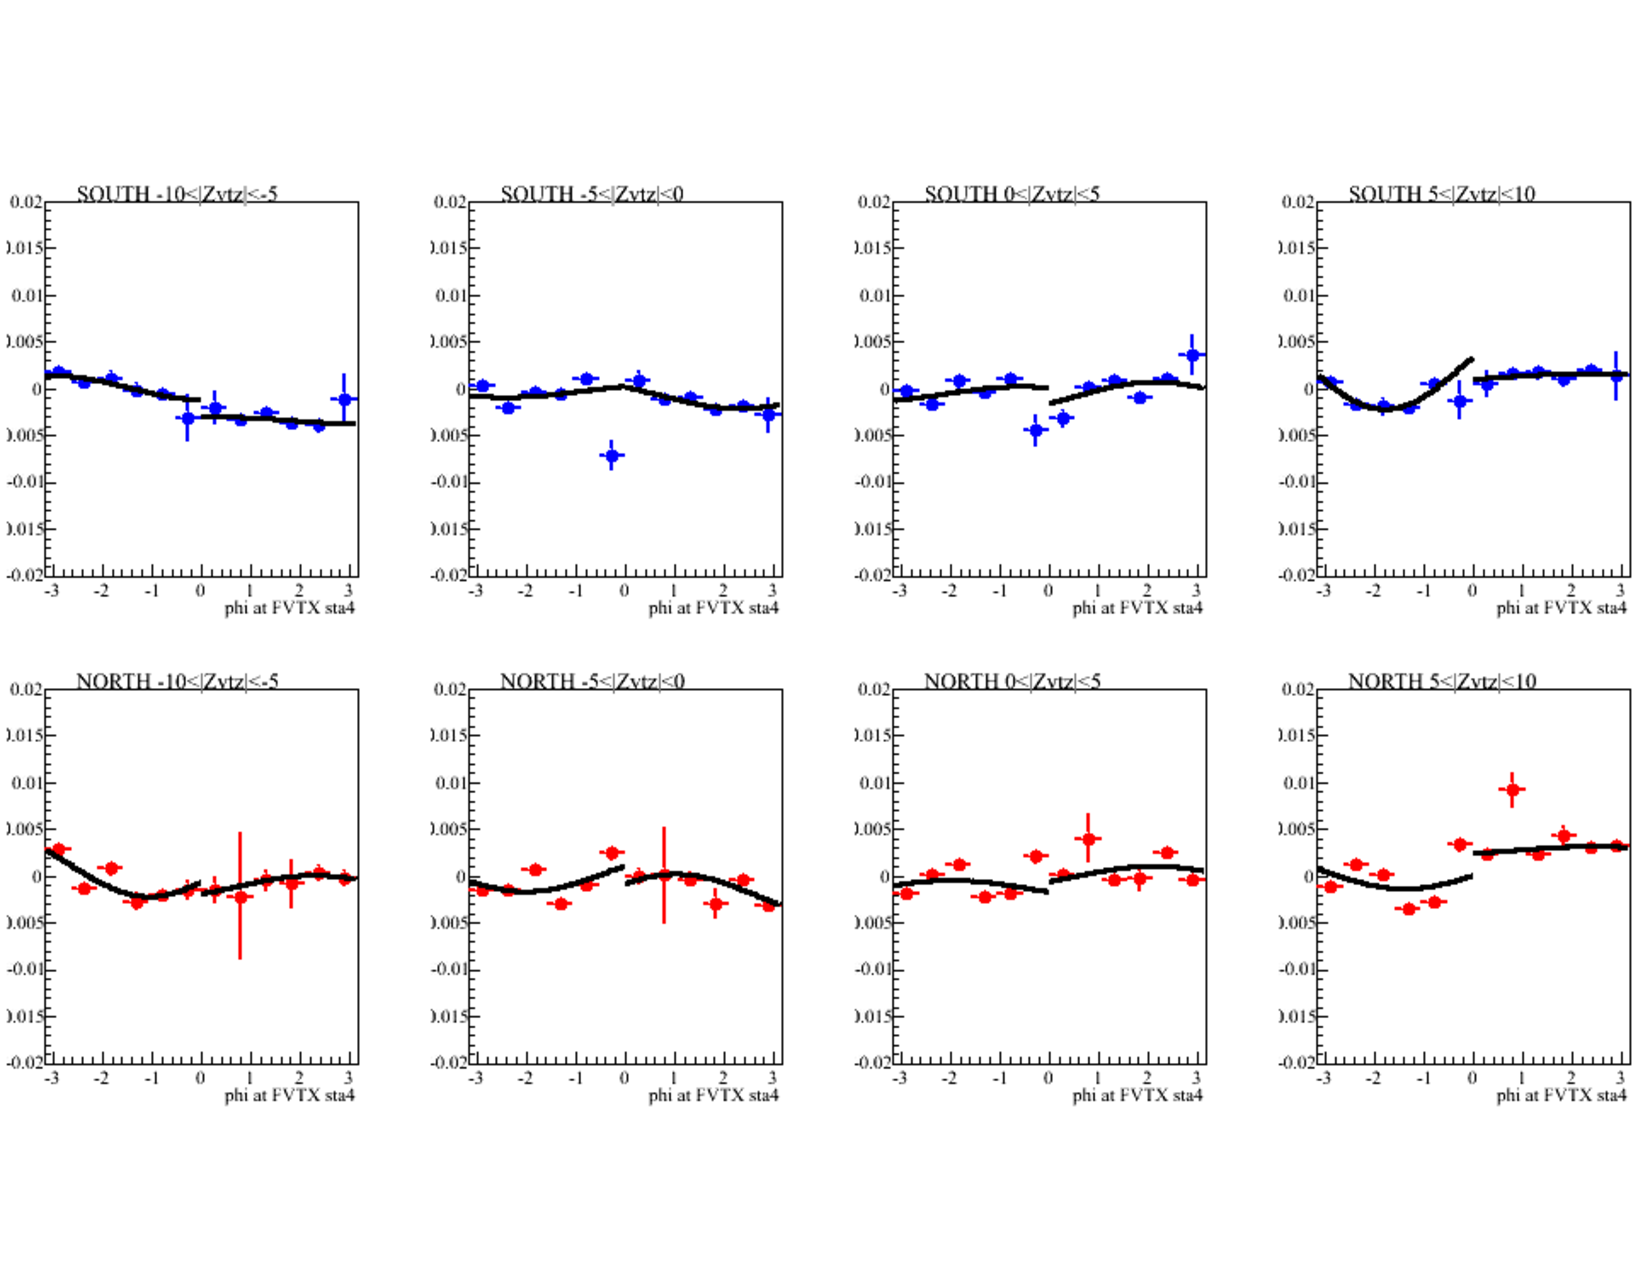
\includegraphics[width=1.0\textwidth]{Figures/dca_phi_after_alignment}
	\caption{\label{fig:dca_phi_after_alignment}Azinuthal dependence of \dcar after post-production alignment.{\color{red} REPLACE ME}}
\end{figure}


%%%%%%%%%%%%%%%%%%%%%%%%%%%%%%%%%%%%%%%%%%%%%%%%%%%%%%%%
\subsection{Fit Procedure}
\label{sec:Fit}

%%%%%%%%%%%%%%%%%%%%%%%%%%%%%%%%%%%%%%%%%%%%%%%%%%%%%%%%
\subsection{Acceptance by efficiency correction}
\label{sec:accbyeff}
For the final ratio calculation, we need to apply relative acceptance by efficiency between prompt \jpsi and \bjpsi events.
\begin{equation}
R_{corrected} = R_{measured}\cdot\frac{\varepsilon_{prompt~J/\psi\to\mu\mu}}{\varepsilon_{B\to J/\psi\to\mu\mu}}
\end{equation}
where $R$ is the ratio of \bjpsi to prompt \jpsi, and $\varepsilon$ is the acceptance by efficiency.
By using simulation done to make sample distribution for the fit, acceptance by efficiencies for prompt \jpsi and \bjpsi are calculated.
Figure~\ref{fig:Jpsi_acceff} shows acceptance by efficiency calculation for prompt \jpsi.
The left and middle panels show generated (red) and reconstructed (black) dimuon's \pt distributions for South and North arm, and the right panel shows final efficiency.
The reconstructed dimuons are passing all analysis cuts in table~\ref{tab:cuts}. 
Figure~\ref{fig:BJpsi_acceff} shows same distributions for \bjpsi events.
A comparison between \jpsi and \bjpsi events are shown in figure~\ref{fig:acceff_comparison}, and the ratio of efficiencies shown in the right panel is a correction factor for measured ratio from the fit.

\begin{figure}[!htb]
	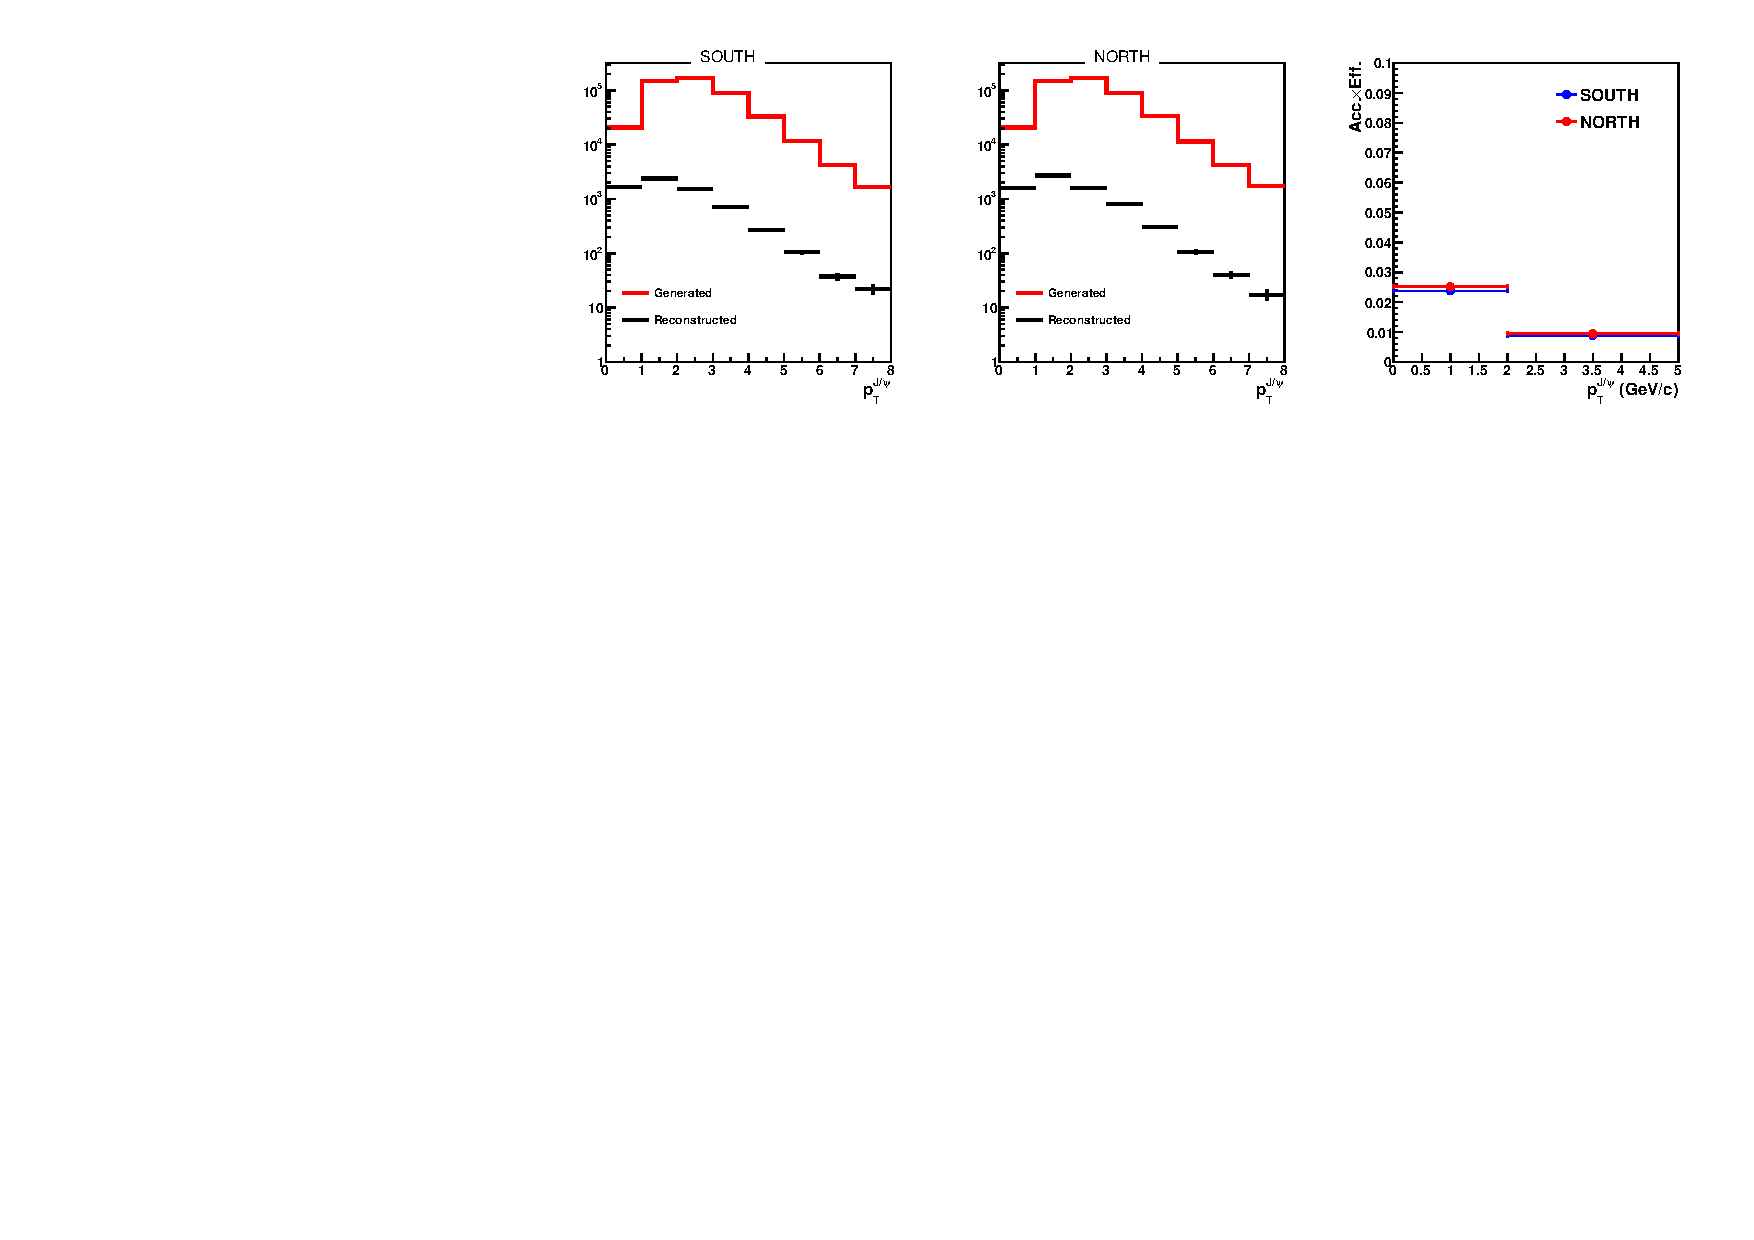
\includegraphics[width=1.0\textwidth]{Figures/Run12pp510_Jpsi_acc_eff}
	\caption{Acceptance by efficiency for prompt \jpsi events}
	\label{fig:Jpsi_acceff}
\end{figure}

\begin{figure}[!htb]
	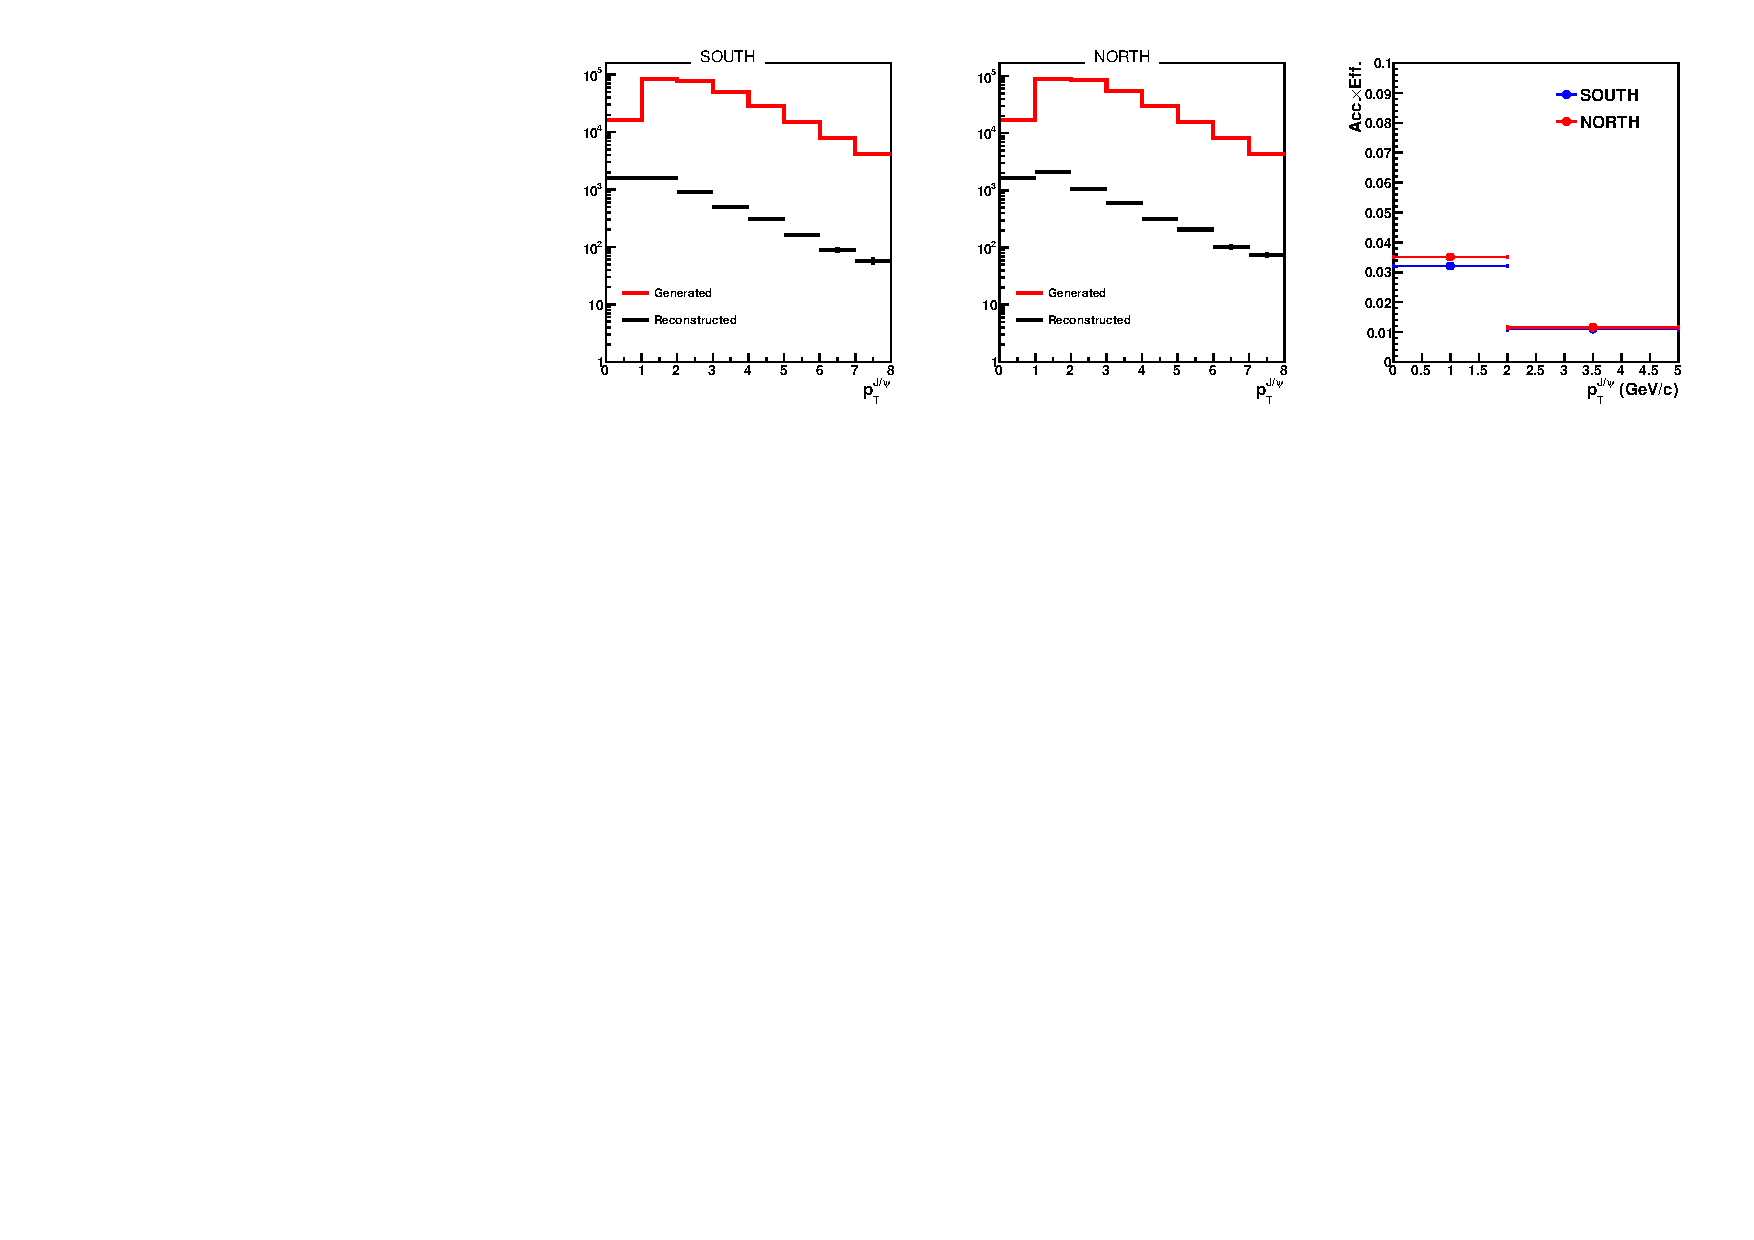
\includegraphics[width=1.0\textwidth]{Figures/Run12pp510_BJpsi_acc_eff}
	\caption{Acceptance by efficiency for \bjpsi events}
	\label{fig:BJpsi_acceff}
\end{figure}

\begin{figure}[!htb]
	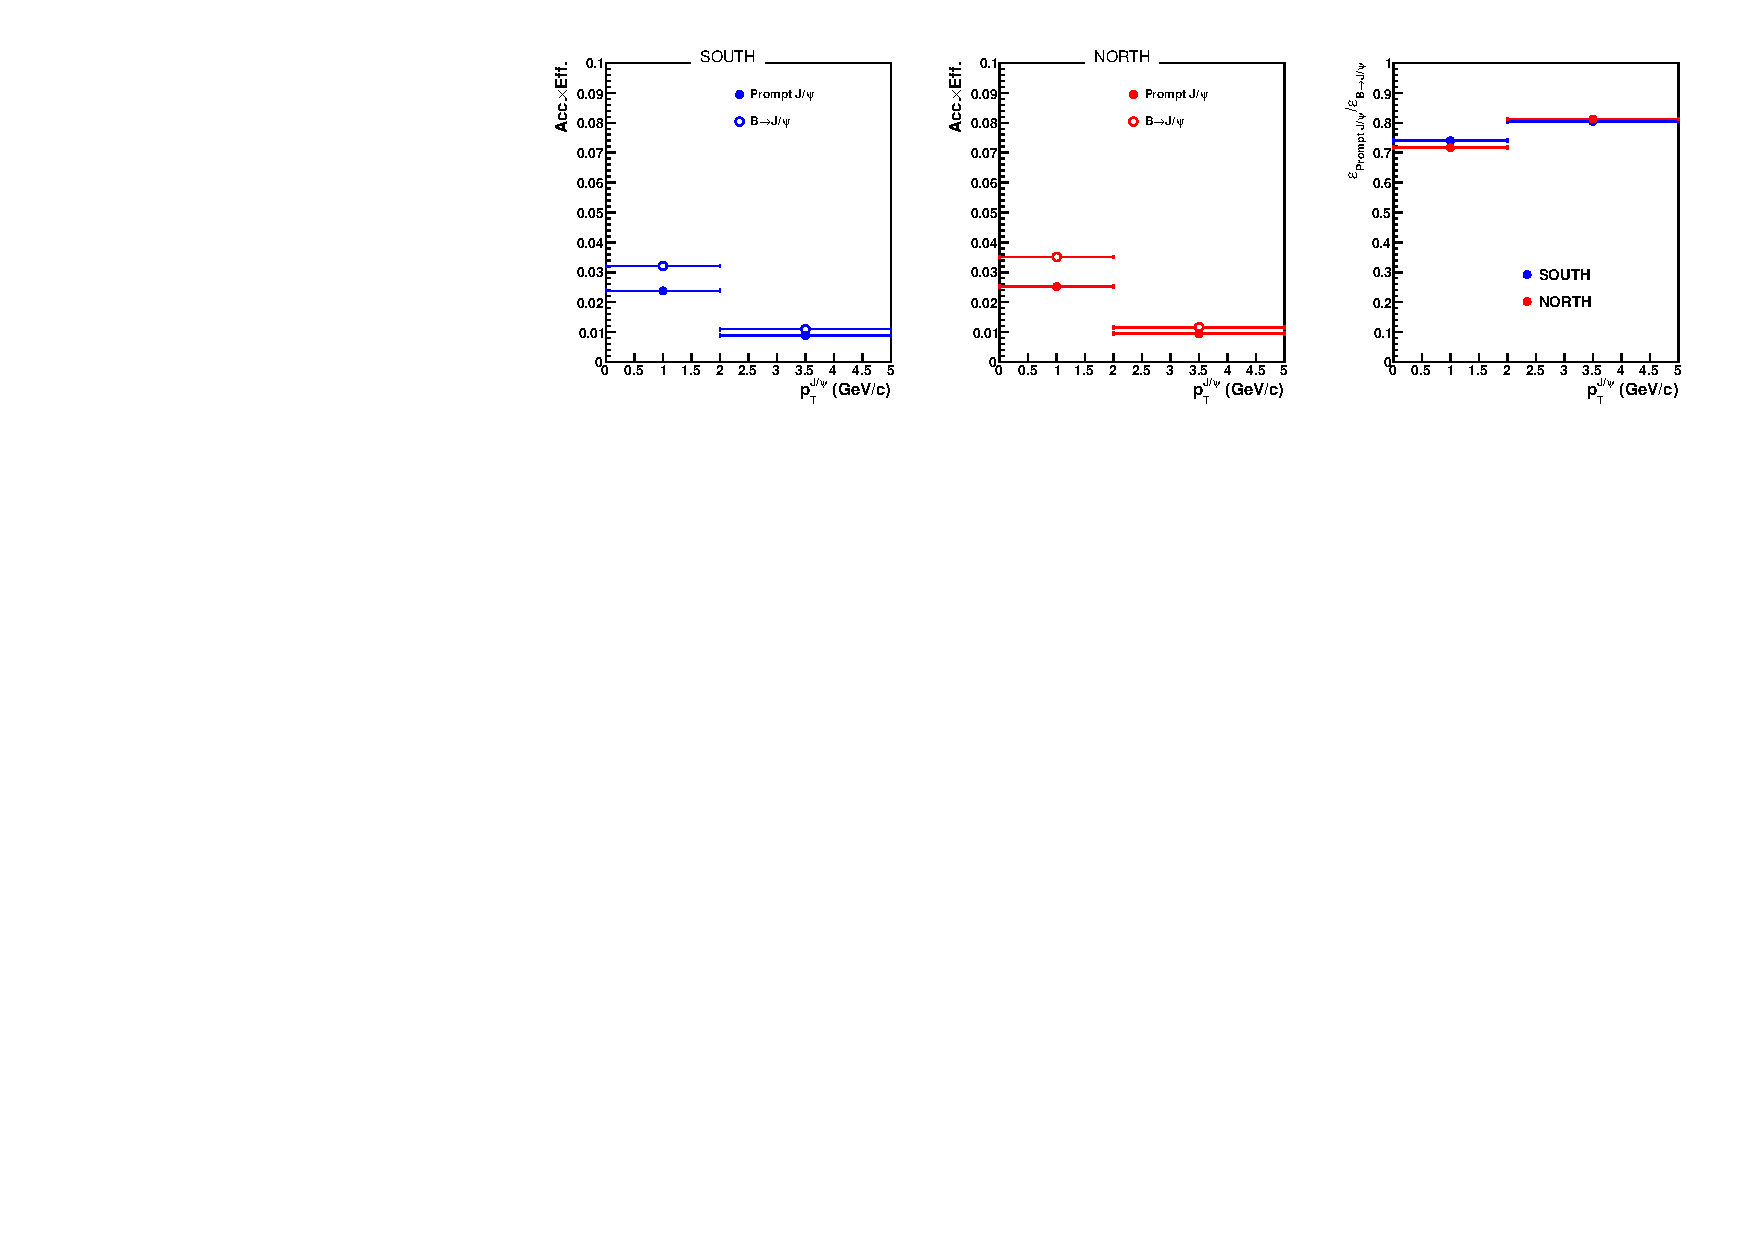
\includegraphics[width=1.0\textwidth]{Figures/Run12pp510_acc_eff_comparison}
	\caption{Comparison of acceptance by efficiency between prompt \jpsi and \bjpsi}
	\label{fig:acceff_comparison}
\end{figure}

\begin{figure}[!htb]
\begin{center}
	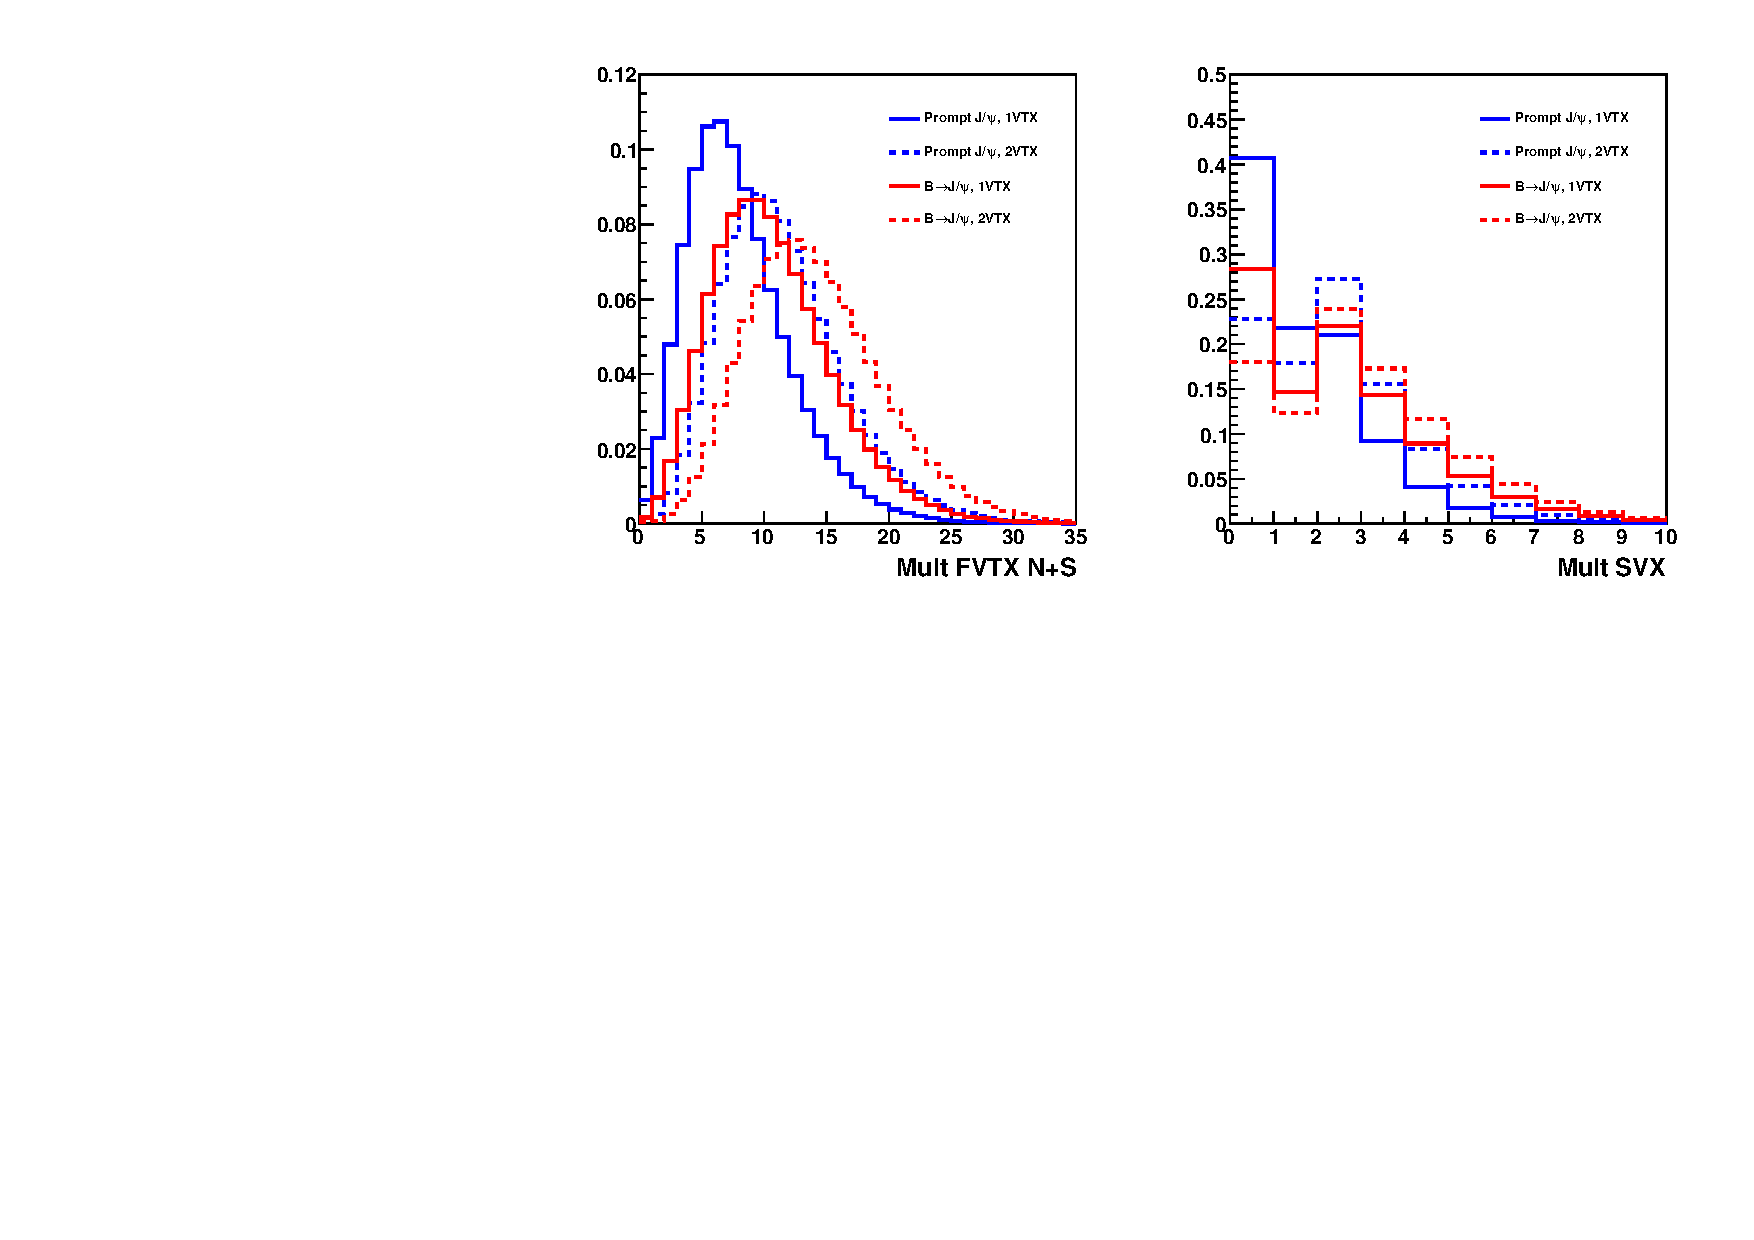
\includegraphics[width=0.8\textwidth]{Figures/Run12pp510_sim_FVTX_SVX_multiplicity}
	\caption{Multiplicity distribution at South and North FVTX (left) and VTX (right).}
	\label{fig:mulitplicity_sim}
\end{center}
\end{figure}

Even though $J/\psi\to\mu\mu$ decay kinematics should be same between prompt \jpsi and \bjpsi, we observed quite different acceptance by efficiency numbers as shown on the right panel in Figure~\ref{fig:acceff_comparison}.
From further investigations to figure out where the difference comes, the probability of \fvtxz reconstruction is 40\% (50\%) for prompt \jpsi (\bjpsi) events which could explain about 20\% difference.
Figure~\ref{fig:mulitplicity_sim} shows multiplicity distributions in FVTX and VTX detectors for prompt \jpsi and \bjpsi events, and the average multiplicity in \bjpsi events is larger than that in prompt \jpsi events.
Particularly on the multiplicity in VTX, there is larger fraction of zero-multiplicity events in prompt \jpsi simulation than \bjpsi simulation.
As discussed in section~\ref{sec:DCA}, \fvtxz reconstruction is largely affected by VTX multiplicity, so the difference observed in acceptance by efficiency can be explained by multiplicity distributions.


%%%%%%%%%%%%%%%%%%%%%%%%%%%%%%%%%%%%%%%%%%%%%%%%%%%%%%%%
\subsection{Systematic Errors}
\label{sec:SystErrors}


%%%%%%%%%%%%%%%%%%%%%%%%%%%%%%%%%%%%%%%%%%%%%%%%%%%%%%%%%%%%
\section{Results}
{\color{red}FIXME}

%%%%%%%%%%%%%%%%%%%%%%%%%%%%%%%%%%%%%%%%%%%%%%%%%%%%%%%%%%%%
\section{Appendix}

\subsection{Good Run List}

365306, 365313, 365330, 365339, 365340, 365342, 365343, 365499, 365500, 365501, 365506,
365513, 365532, 365537, 365538, 365539, 365543, 365544, 365546, 365547, 365551, 365662,
365663, 365671, 365672, 365673, 365675, 365680, 365703, 365711, 365713, 365714, 365718,
365720, 365721, 365723, 365727, 365729, 365841, 365842, 365843, 365845, 365848, 365853,
365854, 365855, 365862, 365863, 365889, 365890, 365891, 365894, 365896, 365897, 365899,
365901, 365902, 365904, 365906, 365912, 365914, 365915, 365916, 365918, 365919, 365922,
365923, 365927, 365928, 365929, 365931, 366033, 366034, 366035, 366036, 366039, 366040,
366041, 366042, 366053, 366054, 366060, 366426, 366427, 366428, 366440, 366586, 366587,
366602, 366632, 366635, 366636, 366637, 366669, 366703, 366788, 366789, 366790, 366793,
366794, 366795, 366796, 366897, 366898, 366899, 366900, 366901, 366902, 366904, 366907,
366910, 366975, 366976, 366977, 366978, 367033, 367034, 367035, 367036, 367037, 367038,
367039, 367062, 367067, 367076, 367099, 367134, 367159, 367161, 367162, 367165, 367166,
367232, 367233, 367234, 367236, 367237, 367238, 367239, 367313, 367316, 367318, 367319,
367320, 367321, 367322, 367323, 367324, 367329, 367330, 367331, 367335, 367336, 367338,
367340, 367341, 367342, 367343, 367345, 367448, 367449, 367450, 367451, 367452, 367453,
367454, 367462, 367463, 367465, 367466, 367467, 367468, 367471, 367510, 367511, 367512,
367513, 367538, 367539, 367543, 367545, 367546, 367548, 367549, 367550, 367552, 367553,
367593, 367594, 367596, 367597, 367598, 367600, 367601, 367602, 367603, 367607, 367608,
367610, 367611, 367612, 367614, 367617, 367620, 367659, 367660, 367662, 367663, 367664,
367665, 367716, 367718, 367720, 367723, 367726, 367727, 367728, 367735, 367737, 367919,
367921, 367923, 367925, 367926, 367927, 367928, 367929, 368037, 368038, 368039, 368040,
368042, 368181, 368183, 368184, 368185, 368186, 368190, 368194, 368206, 368212, 368213,
368217, 368218, 368219, 368223, 368279, 368280, 368338, 368339, 368341, 368344, 368346,
368347, 368356, 368357, 368358, 368359, 368360, 368361, 368364, 368366, 368367, 368368,
368390, 368391, 368393, 368394, 368395, 368407, 368408, 368409, 368410, 368529, 368532,
368533, 368535, 368544, 368545, 368546, 368547, 368621, 368622, 368623, 368624, 368627,
368628, 368629, 368630, 368683, 368686, 368687, 368689, 368690, 368692, 368694, 368695,
368742, 368744, 368786, 368787, 368789, 368790, 368792, 368795, 368797, 368798




\subsection{Data tables}

{\it
  No results without data tables!  List errors separately
  (statistical, type A, B, C) and the total.  If you have many tables,
  breaking them up into subsections is strongly recommended.
}


%%%%%%%%%%%%%%%%%%%%%%%%%%%%%%%%%%%%%%%%%%%%%%%%%%%%%%%%%%%%
\begin{thebibliography}{9}

%\cite{ref:CT10}
\bibitem{ref:CT10} 
  H.~L.~Lai, M.~Guzzi, J.~Huston, Z.~Li, P.~M.~Nadolsky, J.~Pumplin and C.-P.~Yuan,
  %``New parton distributions for collider physics,''
  Phys.\ Rev.\ D {\bf 82}, 074024 (2010)
  [arXiv:1007.2241 [hep-ph]].
  %%CITATION = ARXIV:1007.2241;%%
  %1173 citations counted in INSPIRE as of 24 Feb 2015


%\cite{ref:Geant4}
\bibitem{ref:Geant4} 
  A.~Dellacqua, G.~Parrour, S.~Giani, P.~Kent, A.~Osborne, S.~Ravndal, L.~Silvestris and H.~Fesefeldt {\it et al.},
  %``GEANT-4: An Object oriented toolkit for simulation in HEP,''
  CERN-DRDC-94-29, CERN-DRDC-P58.
  %%CITATION = CERN-DRDC-94-29, CERN-DRDC-P58;%%
  %2 citations counted in INSPIRE as of 24 Feb 2015

\bibitem{ref:PHG3toG4} PHG3toG4
   {\it https://www.phenix.bnl.gov/WWW/offline/wikioff/index.php/PHG3toG4 }

\bibitem{ref:G4ROOT} G4ROOT
   {\it https://root.cern.ch/drupal/content/g4root}
   
\bibitem{ref:an1103} PHENIX analysis note 1103


\end{thebibliography}

\end{document}



